\documentclass[a4paper]{article}

\def\npart {III}
\def\nterm {Lent}
\def\nyear {2018}
\def\nlecturer {J.\ Miller}
\def\ncourse {Schramm--Loewner Evolutions}
\def\nofficial {http://statslab.cam.ac.uk/~jpm205/teaching/lent2018/}

% Imports
\ifx \nextra \undefined
  \usepackage[pdftex,
    hidelinks,
    pdfauthor={Dexter Chua},
    pdfsubject={Cambridge Maths Notes: Part \npart\ - \ncourse},
    pdftitle={Part \npart\ - \ncourse},
  pdfkeywords={Cambridge Mathematics Maths Math \npart\ \nterm\ \nyear\ \ncourse}]{hyperref}
  \title{Part \npart\ - \ncourse}
\else
  \usepackage[pdftex,
    hidelinks,
    pdfauthor={Dexter Chua},
    pdfsubject={Cambridge Maths Notes: Part \npart\ - \ncourse\ (\nextra)},
    pdftitle={Part \npart\ - \ncourse\ (\nextra)},
  pdfkeywords={Cambridge Mathematics Maths Math \npart\ \nterm\ \nyear\ \ncourse\ \nextra}]{hyperref}

  \title{Part \npart\ - \ncourse \\ {\Large \nextra}}
\fi

\author{Lectured by \nlecturer \\\small Notes taken by Dexter Chua}
\date{\nterm\ \nyear}

\usepackage{alltt}
\usepackage{amsfonts}
\usepackage{amsmath}
\usepackage{amssymb}
\usepackage{amsthm}
\usepackage{booktabs}
\usepackage{caption}
\usepackage{enumitem}
\usepackage{fancyhdr}
\usepackage{graphicx}
\usepackage{mathtools}
\usepackage{microtype}
\usepackage{multirow}
\usepackage{pdflscape}
\usepackage{pgfplots}
\usepackage{siunitx}
\usepackage{tabularx}
\usepackage{tikz}
\usepackage{tkz-euclide}
\usepackage[normalem]{ulem}
\usepackage[all]{xy}

\pgfplotsset{compat=1.12}

\pagestyle{fancyplain}
\lhead{\emph{\nouppercase{\leftmark}}}
\ifx \nextra \undefined
  \rhead{
    \ifnum\thepage=1
    \else
      \npart\ \ncourse
    \fi}
\else
  \rhead{
    \ifnum\thepage=1
    \else
      \npart\ \ncourse\ (\nextra)
    \fi}
\fi
\usetikzlibrary{arrows}
\usetikzlibrary{decorations.markings}
\usetikzlibrary{decorations.pathmorphing}
\usetikzlibrary{positioning}
\usetikzlibrary{fadings}
\usetikzlibrary{intersections}
\usetikzlibrary{cd}

\newcommand*{\Cdot}{\raisebox{-0.25ex}{\scalebox{1.5}{$\cdot$}}}
\newcommand {\pd}[2][ ]{
  \ifx #1 { }
    \frac{\partial}{\partial #2}
  \else
    \frac{\partial^{#1}}{\partial #2^{#1}}
  \fi
}

% Theorems
\theoremstyle{definition}
\newtheorem*{aim}{Aim}
\newtheorem*{axiom}{Axiom}
\newtheorem*{claim}{Claim}
\newtheorem*{cor}{Corollary}
\newtheorem*{defi}{Definition}
\newtheorem*{eg}{Example}
\newtheorem*{fact}{Fact}
\newtheorem*{law}{Law}
\newtheorem*{lemma}{Lemma}
\newtheorem*{notation}{Notation}
\newtheorem*{prop}{Proposition}
\newtheorem*{thm}{Theorem}

\renewcommand{\labelitemi}{--}
\renewcommand{\labelitemii}{$\circ$}
\renewcommand{\labelenumi}{(\roman{*})}

\let\stdsection\section
\renewcommand\section{\newpage\stdsection}

% Strike through
\def\st{\bgroup \ULdepth=-.55ex \ULset}

% Maths symbols
\newcommand{\bra}{\langle}
\newcommand{\ket}{\rangle}

\newcommand{\N}{\mathbb{N}}
\newcommand{\Z}{\mathbb{Z}}
\newcommand{\Q}{\mathbb{Q}}
\renewcommand{\H}{\mathbb{H}}
\newcommand{\R}{\mathbb{R}}
\newcommand{\C}{\mathbb{C}}
\newcommand{\Prob}{\mathbb{P}}
\renewcommand{\P}{\mathbb{P}}
\newcommand{\E}{\mathbb{E}}
\newcommand{\F}{\mathbb{F}}
\newcommand{\cU}{\mathcal{U}}
\newcommand{\RP}{\mathbb{RP}}
\newcommand{\CP}{\mathbb{CP}}

\newcommand{\ph}{\,\cdot\,}

\DeclareMathOperator{\sech}{sech}
\DeclareMathOperator{\cosech}{cosech}
\DeclareMathOperator{\cosec}{cosec}

\DeclareMathOperator{\covol}{covol}
\DeclareMathOperator{\vol}{vol}

\let\Im\relax
\let\Re\relax
\DeclareMathOperator{\Im}{Im}
\DeclareMathOperator{\Re}{Re}
\DeclareMathOperator{\im}{im}
\DeclareMathOperator{\image}{image}
\DeclareMathOperator{\Ann}{Ann}

\DeclareMathOperator*{\res}{res}
\DeclareMathOperator{\Res}{Res}
\DeclareMathOperator{\Ind}{Ind}

\DeclareMathOperator{\tr}{tr}
\DeclareMathOperator{\diag}{diag}
\DeclareMathOperator{\rank}{rank}
\DeclareMathOperator{\card}{card}
\DeclareMathOperator{\spn}{span}
\DeclareMathOperator{\adj}{adj}

\DeclareMathOperator{\erf}{erf}
\DeclareMathOperator{\erfc}{erfc}

\DeclareMathOperator{\ord}{ord}
\DeclareMathOperator{\Sym}{Sym}

\DeclareMathOperator{\sgn}{sgn}
\DeclareMathOperator{\orb}{orb}
\DeclareMathOperator{\stab}{stab}
\DeclareMathOperator{\ccl}{ccl}

\DeclareMathOperator{\lcm}{lcm}
\DeclareMathOperator{\hcf}{hcf}

\DeclareMathOperator{\Int}{Int}
\DeclareMathOperator{\id}{id}

\DeclareMathOperator{\betaD}{beta}
\DeclareMathOperator{\gammaD}{gamma}
\DeclareMathOperator{\Poisson}{Poisson}
\DeclareMathOperator{\binomial}{binomial}
\DeclareMathOperator{\multinomial}{multinomial}
\DeclareMathOperator{\Bernoulli}{Bernoulli}
\DeclareMathOperator{\like}{like}

\DeclareMathOperator{\var}{var}
\DeclareMathOperator{\cov}{cov}
\DeclareMathOperator{\bias}{bias}
\DeclareMathOperator{\mse}{mse}
\DeclareMathOperator{\corr}{corr}

\DeclareMathOperator{\otp}{otp}
\DeclareMathOperator{\dom}{dom}

\DeclareMathOperator{\Root}{Root}
\DeclareMathOperator{\supp}{supp}
\DeclareMathOperator{\rel}{rel}
\DeclareMathOperator{\Hom}{Hom}
\DeclareMathOperator{\Aut}{Aut}
\DeclareMathOperator{\Gal}{Gal}
\DeclareMathOperator{\Mat}{Mat}
\DeclareMathOperator{\End}{End}
\DeclareMathOperator{\Char}{char}
\DeclareMathOperator{\ev}{ev}
\DeclareMathOperator{\St}{St}
\DeclareMathOperator{\Lk}{Lk}
\DeclareMathOperator{\disc}{disc}
\DeclareMathOperator{\Isom}{Isom}
\DeclareMathOperator{\length}{length}
\DeclareMathOperator{\energy}{energy}
\DeclareMathOperator{\area}{area}
\DeclareMathOperator{\Syl}{Syl}
\DeclareMathOperator{\cl}{cl}
\DeclareMathOperator{\fix}{fix}

\newcommand{\GL}{\mathrm{GL}}
\newcommand{\SL}{\mathrm{SL}}
\newcommand{\PGL}{\mathrm{PGL}}
\newcommand{\PSL}{\mathrm{PSL}}
\newcommand{\PSU}{\mathrm{PSU}}
\newcommand{\Or}{\mathrm{O}}
\newcommand{\SO}{\mathrm{SO}}
\newcommand{\U}{\mathrm{U}}
\newcommand{\SU}{\mathrm{SU}}

\renewcommand{\d}{\mathrm{d}}
\newcommand{\D}{\mathrm{D}}

\tikzset{->/.style = {decoration={markings,
                                  mark=at position 1 with {\arrow[scale=2]{latex'}}},
                      postaction={decorate}}}
\tikzset{<-/.style = {decoration={markings,
                                  mark=at position 0 with {\arrowreversed[scale=2]{latex'}}},
                      postaction={decorate}}}
\tikzset{<->/.style = {decoration={markings,
                                   mark=at position 0 with {\arrowreversed[scale=2]{latex'}},
                                   mark=at position 1 with {\arrow[scale=2]{latex'}}},
                       postaction={decorate}}}
\tikzset{->-/.style = {decoration={markings,
                                   mark=at position #1 with {\arrow[scale=2]{latex'}}},
                       postaction={decorate}}}
\tikzset{-<-/.style = {decoration={markings,
                                   mark=at position #1 with {\arrowreversed[scale=2]{latex'}}},
                       postaction={decorate}}}

\tikzset{circ/.style = {fill, circle, inner sep = 0, minimum size = 3}}
\tikzset{mstate/.style={circle, draw, blue, text=black, minimum width=0.7cm}}

\definecolor{mblue}{rgb}{0.2, 0.3, 0.8}
\definecolor{morange}{rgb}{1, 0.5, 0}
\definecolor{mgreen}{rgb}{0.1, 0.4, 0.2}
\definecolor{mred}{rgb}{0.5, 0, 0}

\def\drawcirculararc(#1,#2)(#3,#4)(#5,#6){%
    \pgfmathsetmacro\cA{(#1*#1+#2*#2-#3*#3-#4*#4)/2}%
    \pgfmathsetmacro\cB{(#1*#1+#2*#2-#5*#5-#6*#6)/2}%
    \pgfmathsetmacro\cy{(\cB*(#1-#3)-\cA*(#1-#5))/%
                        ((#2-#6)*(#1-#3)-(#2-#4)*(#1-#5))}%
    \pgfmathsetmacro\cx{(\cA-\cy*(#2-#4))/(#1-#3)}%
    \pgfmathsetmacro\cr{sqrt((#1-\cx)*(#1-\cx)+(#2-\cy)*(#2-\cy))}%
    \pgfmathsetmacro\cA{atan2(#2-\cy,#1-\cx)}%
    \pgfmathsetmacro\cB{atan2(#6-\cy,#5-\cx)}%
    \pgfmathparse{\cB<\cA}%
    \ifnum\pgfmathresult=1
        \pgfmathsetmacro\cB{\cB+360}%
    \fi
    \draw (#1,#2) arc (\cA:\cB:\cr);%
}
\newcommand\getCoord[3]{\newdimen{#1}\newdimen{#2}\pgfextractx{#1}{\pgfpointanchor{#3}{center}}\pgfextracty{#2}{\pgfpointanchor{#3}{center}}}

\def\Xint#1{\mathchoice
   {\XXint\displaystyle\textstyle{#1}}%
   {\XXint\textstyle\scriptstyle{#1}}%
   {\XXint\scriptstyle\scriptscriptstyle{#1}}%
   {\XXint\scriptscriptstyle\scriptscriptstyle{#1}}%
   \!\int}
\def\XXint#1#2#3{{\setbox0=\hbox{$#1{#2#3}{\int}$}
     \vcenter{\hbox{$#2#3$}}\kern-.5\wd0}}
\def\ddashint{\Xint=}
\def\dashint{\Xint-}

\renewcommand\D{\mathbb{D}}
\DeclareMathOperator\hcap{hcap}
\newcommand\SLE{\mathrm{SLE}}
\newcommand\rad{\mathrm{Rad}}
\newcommand\dist{\mathrm{dist}}
\newcommand\BES{\mathrm{BES}}

\usepackage[first=0,last=1, seed=173]{lcg}
%\usepackage{mathrsfs}

\pdfmapline{=stix-mathscr STIXMathScript-Regular " -.25 SlantFont " <stix-mathscr.pfb}
\DeclareFontEncoding{LS1}{}{}
\DeclareFontSubstitution{LS1}{stix}{m}{n}
\DeclareMathAlphabet{\mathscr}{LS1}{stixscr}{m}{n}

\begin{document}
\maketitle
{\small
\setlength{\parindent}{0em}
\setlength{\parskip}{1em}
Schramm--Loewner Evolution (SLE) is a family of random curves in the plane, indexed by a parameter $\kappa \geq 0$. These non-crossing curves are the fundamental tool used to describe the scaling limits of a host of natural probabilistic processes in two dimensions, such as critical percolation interfaces and random spanning trees. Their introduction by Oded Schramm in 1999 was a milestone of modern probability theory.

The course will focus on the definition and basic properties of SLE. The key ideas are conformal invariance and a certain spatial Markov property, which make it possible to use It\^o calculus for the analysis. In particular we will show that, almost surely, for $\kappa \leq 4$ the curves are simple, for $4 \leq \kappa < 8$ they have double points but are non-crossing, and for $\kappa \geq 8$ they are space-filling. We will then explore the properties of the curves for a number of special values of $\kappa$ (locality, restriction properties) which will allow us to relate the curves to other conformally invariant structures.

The fundamentals of conformal mapping will be needed, though most of this will be developed as required. A basic familiarity with Brownian motion and It\^o calculus will be assumed but recalled.
}
\tableofcontents

\setcounter{section}{-1}
\section{Introduction}
Schramm--Loewner evolution is a random curve in a complex domain $D$ (which we will often take to be $\H$ for convenience), parametrized by a positive real number $\kappa$. This was introduced by Schramm in 1999 to describe various scaling limits that arise in probability theory and statistical physics.

Recall that if we take a random walk on the integer lattice $\Z^d$, and take the scaling limit as the grid size tends to $0$, we converge towards a Brownian motion. There are other discrete models that admit a scaling limit, and the limit is often something that is not Brownian motion.

Schramm showed that if the scaling limit satisfies certain conformal invariance properties, which many models do, then it must be $\SLE_\kappa$ for some $\kappa$. If we can identify exactly which $\kappa$ it belongs to, then this will completely determine what the scaling limit is, and often conveys a lot of extra information such as the critical exponents. This has been done for several discrete models:
\begin{itemize}
  \item The scaling limit of loop-erased random walk is $\SLE_2$
  \item The scaling limit of hexagonal percolation is $\SLE_6$ (see chapter \ref{sec:percolation})
  \item It is conjectured that the scaling limit of self-avoiding random walk is $\SLE_{8/3}$ (see chapter \ref{sec:saw})
  \item The ``level sets'' of a Gaussian free field are $\SLE_4$'s (see chapter\ref{sec:gff}).
\end{itemize}
In this course, we will prove some basic properties of $\SLE_\kappa$, and then establish the last three results/conjectures.

\section{Conformal transformations}
\subsection{Conformal transformations}
\begin{defi}[Conformal map]\index{conformal map}
  Let $U, V$ be domains in $\C$. We say a holomorphic function $f: U \to V$ is \emph{conformal} if it is a bijection.
\end{defi}

We will write \term{$\D$} for the open unit disk, and \term{$\H$} for the upper half plane. An important theorem about conformal maps is the following:
\begin{thm}[Riemann mapping theorem]
  Let $U$ be a simply connected domain with $U \not= \C$ and $z \in U$ be any point. Then there exists a unique conformal transformation $f: \D \to U$ such that $f(0) = z$, and $f'(0)$ is real and positive.
\end{thm}
We shall not prove this theorem, as it is a standard result. An immediate corollary is that any two simply connected domains that are distinct from $\C$ are conformally equivalent.

\begin{eg}
  Take $U = \D$. Then for $z \in \D$, the map promised by the Riemann mapping theorem is
  \[
    f(w) = \frac{w + z}{1 + \bar{z} w}.
  \]
  In general, every conformal transformation $f: \D \to \D$ is of the form
  \[
    f(w) = \lambda \frac{w + z}{1 + \bar{z}w}
  \]
  for some $|\lambda| = 1$ and $z \in \D$.
\end{eg}

\begin{eg}
  The map $f: \H \to \D$ given by
  \[
    f(z) = \frac{z - i}{z + i},
  \]
  is a conformal transformation, with inverse
  \[
    g(w) = \frac{i(1 + w)}{1 - w}.
  \]
  In general, the conformal transformations $\H \to \H$ consist of maps of the form
  \[
    f(z) = \frac{az + b}{c z + d}
  \]
  with $a, b, c, d \in \R$ and $ad - bc \not= 0$.
\end{eg}

\begin{eg}
  For $t \geq 0$, we let $H_t = \H \setminus [0, 2\sqrt{t} i]$. The map $H_t \to \H$ given by
  \[
    z \mapsto \sqrt{z^2 + 4t}
  \]
  is a conformal transformation. Observe that this map satisfies
  \[
    |g_t(z) - z| = |\sqrt{z^2 + 4t} - z| \to 0\text{ as } z \to \infty.
  \]
  So $g_t(z) \sim z$ for large $z$.

  Observe also that the family $g_t(z)$ satisfies the ODE
  \[
    \frac{\partial g}{\partial t} = \frac{2}{g_t(z)},\quad g_0(z) = z.
  \]
  We can think of these functions $g_t$ as being generated by the curve $\gamma(t) = 2 \sqrt{t}i$, where for each $t$, the function $g_t$ is the conformal transformation that sends $\H \setminus \gamma([0, t])$ to $\H$ (satisfying $|g_t(z) - z| \to \infty$).

  Given the set of functions $g_t$, we can recover the curve $\gamma$ as follows --- for each $z \in \H$, we can ask what is the minimum $t$ such that $g_t$ is not defined on $z$. By ODE theorems, there is a solution up till the point when $g_t(z) = 0$, in which case the denominator of the right hand side blows up. Call this time $\tau(z)$. We then see that for each $t$, there is a unique $z$ such that $\tau(z) = t$, and we have $\gamma(t) = z$.

  More generally, suppose $\gamma$ is any simple (i.e.\ non-self-intersecting) curve in $\H$ starting from $0$. Then for each $t$, we can let $g_t$ be the unique conformal transformation that maps $\H \setminus \gamma([0, t])$ to $\H$ with $|g_t(z) - z| \to \infty$ as above (we will later see such a map exists). Then \emph{Loewner's theorem} says there is a continuous, real-valued function $W$ such that
  \[
    \frac{\partial g_t}{\partial t} = \frac{2}{g_t(z) - W_t},\quad g_0(z) = z.
  \]
  This is the \term{chordal Loewner equation}. We can turn this around --- given a function $W_t$, what is the corresponding curve $\gamma(t)$? If $W = 0$, then $\gamma(t) = 2\sqrt{t}i$. More excitingly, if we take $W_t = \sqrt{\kappa} B_t$, where $B_t$ is a standard Brownian motion, and interpret this equation as a stochastic differential equation, we obtain $\SLE_\kappa$.
\end{eg}
\subsection{Brownian motion and harmonic functions}
Recall that a function $f = u + iv$ is holomorphic iff it satisfies the \term{Cauchy--Riemann equations}
\[
  \frac{\partial u}{\partial x} = \frac{\partial v}{\partial y},\quad \frac{\partial u}{\partial y} = - \frac{\partial v}{\partial x}.
\]
This in particular implies that both $u$ and $v$ are \term{harmonic}.
\begin{defi}[Harmonic function]\index{harmonic function}
  A function $f: \R^k \to \R$ is \emph{harmonic} if it is $C^2$ and
  \[
    \Delta f = \left(\frac{\partial^2}{\partial x_1^2} + \cdots + \frac{\partial^2}{\partial x_k^2}\right) f = 0.
  \]
\end{defi}
Indeed, we can calculate
\[
  \frac{\partial^2 u}{\partial x^2} + \frac{\partial^2 u}{\partial y^2} = \frac{\partial}{\partial x} \frac{\partial v}{\partial y} + \frac{\partial}{\partial y} \left(- \frac{\partial v}{\partial x}\right) = 0.
\]
In Advanced Probability, we saw that Brownian motion is very closely related to harmonic functions.
\begin{defi}[Complex Brownian motion]
  We say a process $B = B^1 + i B^2$ is a \term{complex Brownian motion} if $(B^1, B^2)$ is a standard Brownian motion in $\R^2$.
\end{defi}

Recall some results from Advanced Probability:
\begin{thm}
  Let $u$ be a harmonic function on a bounded domain $D$ which is continuous on $\bar{D}$. For $z \in D$, let $\P_z$ be the law of a complex Brownian motion starting from $z$, and let $\tau$ be the first hitting time of $D$. Then
  \[
    u(z) = \E_z[u(B_\tau)].\fakeqed
  \]
\end{thm}

\begin{cor}[Mean value property]\index{mean value property}
  If $u$ is a harmonic function, then, whenever it makes sense, we have
  \[
    u(z) = \frac{1}{2\pi} \int_0^{2\pi} u(z + re^{i\theta})\;\d \theta.\qedhere
  \]
\end{cor}
\begin{cor}[Maximum principle]\index{maximum principle}
  Let $u$ be harmonic in a domain $D$. If $u$ attains its maximum at an interior point in $D$, then $u$ is constant.
\end{cor}

\begin{cor}[Maximum modulus principle]\index{maximum modulus principle}
  Let $D$ be a domain and let $f: D \to \C$ be holomorphic. If $|f|$ attains its maximum in the interior of $D$, then $f$ is constant.
\end{cor}

\begin{proof}
  Observe that if $f$ is holomorphic, then $\log |f|$ is harmonic and attains its maximum in the interior of $D$. It then follows that $|f|$ is constant (if $|f|$ vanishes somewhere, then consider $\log |f + M|$ for some large $M$, and do some patching if necessary). It is then a standard result that a holomorphic function of constant modulus is constant.
\end{proof}

The following lemma should be familiar from the old complex analysis days as well:
\begin{lemma}[Schwarz lemma]\index{Schwarz lemma}
  Let $f: \D \to \D$ be a holomorphic map with $f(0) = 0$. Then $|f(z)| \leq |z|$ for all $z \in \D$. If $|f(z)| = |z|$ for some non-zero $z \in \D$, then $f(w) = \lambda w$ for some $\lambda \in \C$ with $|\lambda| = 1$.
\end{lemma}

\begin{proof}
  Consider the map
  \[
   g(z) =
    \begin{cases}
      f(z)/z & z \not =0\\
      f'(0) & z = 0
    \end{cases}.
  \]
  Then one sees that $g$ is holomorphic and $|g(z)| \leq 1$ for all $z \in \partial\D$, hence for all $z \in \D$ by the maximum modulus principle. If $|f(z_0)| = |z_0|$ for some $z_0 \in \D \setminus \{0\}$, then $g$ must be constant, so $f$ is linear.
\end{proof}

\subsection{Distortion estimates for conformal maps}

We write $\mathcal{U}$\index{$\mathcal{U}$} for the collection of conformal transformations $f: \D \to D$, where $D$ is any simply connected domain with $0 \in D$ and $D \not= \C$, with $f(0) = 0$ and $f'(0) = 1$. Thus, it must be of the form
\[
  f(z) = z + \sum_{n = 2}^\infty a_n z^n.
\]
\begin{thm}[Koebe-1/4 theorem]\index{Koebe-1/4 theorem}
  If $f \in \mathcal{U}$ and $0 < r \leq 1$, then $B(0, r/4) \subseteq f(r\D)$.
\end{thm}
This says $f$ cannot look like this:
\begin{center}
  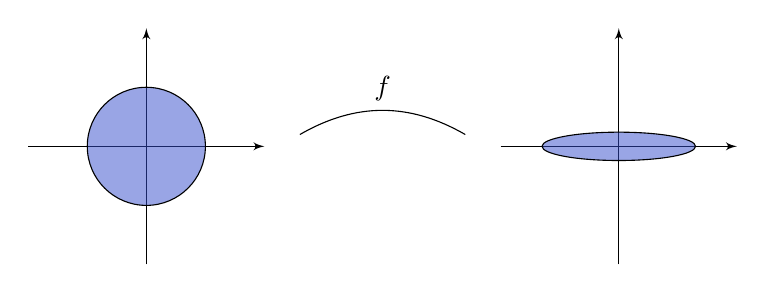
\begin{tikzpicture}[scale=1.5]
    \draw [-latex'] (-1, 0) -- (1, 0);
    \draw [-latex'] (0, -1) -- (0, 1);

    \draw [fill=mblue, fill opacity=0.5] circle [radius=0.5];

    \draw (1.3, 0.1) edge [bend left, ->] node [pos=0.5, above] {$f$} (2.7, 0.1);

    \draw [-latex'] (3, 0) -- (5, 0);
    \draw [-latex'] (4, -1) -- (4, 1);
    \draw [fill=mblue, fill opacity=0.5] (4, 0) ellipse (0.65 and 0.12);
  \end{tikzpicture}
\end{center}
By scaling it suffices to prove this for the case $r = 1$. This follows from the following result:
\begin{thm}
  If $f \in \mathcal{U}$, then $|a_2| \leq 2$.
\end{thm}
The proof of this proposition will involve quite some work. So let us just conclude the theorem from this.
\begin{proof}[Proof of Koebe-1/4 theorem]
  Suppose $f: \D \to D$ is in $\mathcal{U}$, and $z_0 \not \in D$. We shall show that $|z_0| \geq \frac{1}{4}$. Consider the function
  \[
    \tilde{f}(z) = \frac{z_0 f(z)}{z_0 - f(z)}.
  \]
  Since $\tilde{f}$ is composition of conformal transformations, it is itself conformal, and a direct computation shows $\tilde{f} \in \mathcal{U}$. Moreover, if
  \[
    f(z) = z + a_2 z^2 + \cdots,
  \]
  then
  \[
    \tilde{f}(z) = z + \left(a_2 + \frac{1}{z_0}\right)z^2 + \cdots.
  \]
  So we obtain the bounds
  \[
    |a_2|, \left|a_2 + \frac{1}{z_0}\right| \leq 2.
  \]
  By the triangle inequality, we must have $|z_0^{-1}| \leq 4$, hence $|z_0| \geq \frac{1}{4}$.
\end{proof}

The 1/4 theorem bounds the distortion in terms of the value of $f'(0)$. Conversely, if we know how much the distortion is, we can use the theorem to derive bounds on $f'(0)$.
\begin{cor}
  Let $D, \tilde{D}$ be domains and $z \in D$, $\tilde{z} \in \tilde{D}$. If $f: D \to \tilde{D}$ is a conformal transformation with $f(z) = \tilde{z}$, then
  \[
    \frac{\tilde{d}}{4d} \leq |f'(z)| \leq \frac{4\tilde{d}}{d},
  \]
  where $d = \dist(z, \partial D)$ and $\tilde{d} = \dist(\tilde{z}, \partial \tilde{D})$.
\end{cor}

\begin{proof}
  By translation, scaling and rotation, we may assume that $z = \tilde{z} = 0$, $d = 1$ and $f'(0) = 1$. Then we have
  \[
    \tilde{D} = f(D) \supseteq f(\D) \supseteq B(0, 1/4).
  \]
  So $\tilde{d} \geq \frac{1}{4}$, as desired. The other bound follows by considering $f^{-1}$.
\end{proof}
We now proceed to prove the theorem. We first obtain a bound on area, using IA Vector Calculus:
\begin{prop}
  Let $f \in \mathcal{U}$. Then
  \[
    \area(f(\D)) = \pi \sum_{n = 1}^\infty n |a_n|^2.
  \]
\end{prop}

\begin{proof}
  In the ideal world, we will have something that helps us directly compute $\area(f(\D))$. However, for the derivation to work, we need to talk about what $f$ does to the boundary of $\D$, but that is not necessarily well-defined. So we compute $\area(f(r\D))$ for $r < 1$ and then take the limit $r \to 1$.

  So fix $r \in (0, 1)$, and define the curve $\gamma(\theta) = f(re^{i\theta})$ for $\theta \in [0, 2\pi]$. Then we can compute
  \begin{align*}
    \frac{1}{2i} \int_\gamma \bar{z} \;\d z &= \frac{1}{2i} \int_\gamma (x - iy) (\d x + i\;\d y)\\
    &= \frac{1}{2i} \int_\gamma (x - iy) \;\d x + (ix + y)\;\d y\\
    &= \frac{1}{2i} \iint_{f(r\D)} 2i\;\d x\;\d y\\
    &= \area(f(r\D)),
  \end{align*}
  using Green's theorem. We can also compute the left-hand integral directly as
  \begin{align*}
    \frac{1}{2i} \int_\gamma \bar{z}\;\d z &= \frac{1}{2i} \int_0^{2\pi} \overline{f(re^{i\theta})} f'(re^{i\theta}) i re^{i\theta }\;\d \theta\\
    &= \frac{1}{2i} \int_0^{2\pi} \left(\sum_{n = 1}^\infty \bar{a}_n r^n e^{-i\theta n}\right) \left(\sum_{n = 1}^\infty a_n nr^{n - 1} e^{i\theta (n - 1)}\right) ir e^{i\theta}\;\d \theta\\
    &= \pi \sum_{n = 1}^\infty r^{2n} |a_n|^2 n.\qedhere
  \end{align*}
\end{proof}

\begin{defi}[Compact hull]\index{compact hull}
  A \emph{compact hull} is a connected compact set $K \subseteq \C$ with more than one point such that $\C \setminus K$ is connected.
\end{defi}

We want to obtain a similar area estimate for compact hulls. By the Riemann mapping theorem, if $K$ is a compact hull, then there exists a unique conformal transformation $F: \C \setminus \bar{\D}$ to $\C \setminus K$ that fixes infinity and has positive derivative at $\infty$, i.e.\ $\lim\limits_{z \to \infty} F(z)/z > 0$. Let $\mathcal{H}$ be the set of compact hulls containing $0$ with $\lim\limits_{z\to \infty} F(z)/z = 1$. If $K \in \mathcal{H}$, then the Laurent expansion of the corresponding $F$ is
\[
  F(z) = z + b_0 + \sum_{n = 1}^\infty \frac{b_n}{z^n}.
\]
Observe there is a correspondence between the space of such $F$ and $\mathcal{U}$ by sending $F$ to $1/F(1/z)$, and vice versa.
\begin{prop}
  If $K \in \mathcal{H}$, then
  \[
    \area (K) = \pi \left(1 - \sum_{n = 1}^\infty n|b_n|^2\right).
  \]
\end{prop}
Observe that the area is always non-negative. So in particular, we obtain the bound
\[
  \sum_{n = 1}^\infty n |b_n|^2 \leq 1.
\]
In particular, $|b_1| \leq 1$. This will be how we ultimately bound $|a_2|$.
\begin{proof}
  The proof is essentially the same as last time. Let $r > 1$, and let $K_r = F(r \bar{\D})$ (or, if you wish, $\C \setminus F(\C \setminus r\bar{\D})$), and $\gamma(\theta) = F(r e^{i\theta})$. As in the previous proposition, we have
  \begin{align*}
    \area(K_r) &= \frac{1}{2i} \int_\gamma \bar{z} \;\d z\\
    &= \frac{1}{2i} \int_0^{2\pi} \overline{F(re^{i\theta})}F'(re^{i\theta}) ir e^{i\theta}\;\d \theta\\
    &= \pi \left(r^2 - \sum_{n = 1}^\infty n |b_n|^2 r^{-2n}\right).
  \end{align*}
  Then take the limit as $r \to 1$.
\end{proof}
By the correspondence we previously noted, this gives us some estimates on the coefficients of any $f \in \mathcal{U}$. It turns out applying this estimate directly is not good enough. Instead, we want to take the square root of $f(z^2)$.

\begin{lemma}
  Let $f \in \mathcal{U}$. Then there exists an odd function $h \in \mathcal{U}$ with $h(z)^2 = f(z^2)$.
\end{lemma}

\begin{proof}
  Note that $f(0) = 0$ by assumption, so taking the square root can potentially be problematic, since $0$ is a branch point. To get rid of the problem, define the function
  \[
    \tilde{f}(z) =
    \begin{cases}
      \frac{f(z)}{z} & z \not =0\\
      f'(0) & z = 0
    \end{cases}.
  \]
  Then $\tilde{f}$ is non-zero and conformal in $\D$, and so there is a function $g$ with $g(z)^2 = \tilde{f}(z)$. We then set
  \[
    h(z) = z g(z^2).
  \]
  Then $h$ is odd and $h^2 = z^2 g(z^2)^2 = f(z^2)$. It is also immediate that $h(0) = 0 $ and $h'(0) = 1$. We need to show $h$ is injective on $\D$. If $z_1, z_2 \in \D$ with $h(z_1) = h(z_2)$, then
  \[
    z_1 g(z_1^2) = z_2 g(z_2^2).\tag{$*$}
  \]
  By squaring, we know
  \[
    z_1^2 \tilde{f}(z_1^2) = z_2^2 \tilde{f}(z_2)^2.
  \]
  Thus, $f(z_1^2) = f(z_2^2)$ and so $z_1^2 = z_2^2$. But then $(*)$ implies $z_1 = z_2$. So $h$ is injective, and hence $h \in \mathcal{U}$.
\end{proof}

We can now prove the desired theorem.
\begin{proof}[Proof of theorem]
  We can Taylor expand
  \[
    h(z) = z + c_3 z^3 + c_5 z^5 + \cdots.
  \]
  Then comparing $h(z)^2 = f(z^2)$ implies
  \[
    c_3 = \frac{a_2}{2}.
  \]
  Setting $g(z) = \frac{1}{h(1/z)}$, we find that the $z^{-1}$ coefficient of $g$ is $-\frac{a_2}{2}$, and as we previously noted, this must be $\leq 1$.
\end{proof}
\subsection{Half-plane capacity}

\begin{defi}[Compact $\H$-hull]\index{compact $\H$-hull}
  A set $A \subseteq \H$ is called a \emph{compact $\H$-hull} if $A$ is compact, $A = \H \cap \bar{A}$ and $\H \setminus A$ is simply connected. We write $\mathcal{Q}$\index{$\mathcal{Q}$} for the collection of compact $\H$-hulls.
\end{defi}
A large part of the course will be about studying families of compact $\H$-hulls, and in particular random families of compact $\H$-hulls. In this chapter, we will establish some basic results about compact $\H$-hulls, in preparation for Loewner's theorem in the next chapter. We begin with the following important proposition:

\begin{prop}
  For each $A \in \mathcal{Q}$, there exists a unique conformal transformation $g_A: \H \setminus A \to \H$ with $|g_A(z) - z| \to 0$ as $z \to \infty$.
\end{prop}

This conformal transformation $g_A$ will be key to understanding compact $\H$-hulls. The proof of this requires the following theorem:
\begin{thm}[Schwarz reflection principle]\index{Schwarz reflection principle}
  Let $D \subseteq \H$ be a simply connected domain, and let $\phi: D \to \H$ be a conformal transformation which is bounded on bounded sets and sends $\R \cap D$ to $\R$. Then $\phi$ extends by reflection to a conformal transformation on
  \[
    D^* = D \cup \{\bar{z} : z \in D\} = D \cup \bar{D}
  \]
  by setting $\phi(\bar{z}) = \overline{\phi(z)}$.\fakeqed
\end{thm}

\begin{proof}[Proof of proposition]
  The Riemann mapping theorem implies that there exists a conformal transformation $g: \H \setminus A \to \H$. Then $g(z) \to \infty$ as $z \to \infty$. By the Schwarz reflection principle, extend $g$ to a conformal transformation defined on $\C \setminus (A \cup \bar{A})$.

  By Laurent expanding $g$ at $\infty$, we can write
  \[
    g(z) = \sum_{n = -\infty}^N b_{-N} z^N.
  \]
  Since $g$ maps the real line to the real line, all $b_i$ must be real. Moreover, by injectivity, considering large $z$ shows that $N = 1$. In other words, we can write
  \[
    g(z) = b_{-1} z + b_0 + \sum_{n = 1}^\infty \frac{b_n}{z^n},
  \]
  with $b_{-1} \not= 0$. We can then define
  \[
    g_A(z) = \frac{g(z) - b_0}{b_{-1}}.
  \]
  Since $b_0$ and $b_{-1}$ are both real, this is still a conformal transformation, and $|g_A(z) - z| \to 0$ as $z \to \infty$.

  To show uniqueness, suppose $g_A, g_A'$ are two such functions. Then $g_A' \circ g_A^{-1}: \H \to \H$ is such a function for $A = \emptyset$. Thus, it suffices to show that if $g: \H \to \H$ is a conformal mapping such that $g(z) - z \to 0$ as $z \to \infty$, then in fact $g = z$. But we can expand $g(z) - z$ as
  \[
    g(z) - z = \sum_{n = 1}^\infty \frac{c_n}{z^n},
  \]
  and this has to be holomorphic at $0$. So $c_n = 0$ for all $n$, and we are done.
\end{proof}

\begin{defi}[Half-plane capacity]\index{half-plane capacity}
  Let $A \in \mathcal{Q}$. Then the \emph{half-plane capacity} of $A$ is defined to be
  \[
    \hcap(A) = \lim_{z \to \infty} z(g_A(z) - z).
  \]
  Thus, we have
  \[
    g_A(z) = z + \frac{\hcap(A)}{z} + \sum_{n = 2}^\infty \frac{b_n}{z^n}.
  \]
\end{defi}

To justify the name ``capacity'', $\hcap(A)$ had better be non-negative and increasing in $A$. These are both true, as we will soon prove. However, let us first look at some examples.

\begin{eg}
  $z \mapsto \sqrt{z^2 + 4t}$ is the unique conformal transformation $\H \setminus [0, \sqrt{t}i] \to \H$ with $|\sqrt{z^2 + 4z} - z| \to 0$ as $z \to \infty$. We can expand
  \[
    \sqrt{z^2 + 4t} = z + \frac{2t}{z} + \cdots.
  \]
  Thus, we know that $\hcap([0, 2\sqrt{t} i]) = 2t$. This justifies our previous funny parametrization of $[0, \sqrt{t} i]$.
\end{eg}

\begin{eg}
  The map $z \mapsto z + \frac{1}{z}$ maps $\H \setminus \bar{\D} \to \H$. Again, we have $\left|z + \frac{1}{z} - z\right| \to 0$ as $z \to \infty$, and so $\hcap(\H \cap \bar{D}) = 1$.
\end{eg}

\begin{prop}\leavevmode
  \begin{enumerate}
    \item Scaling: If $r > 0$ and $A \in \mathcal{Q}$, then $\hcap(rA) = r^2 \hcap(A)$.
    \item Translation invariance: If $x \in \R$ and $a \in \mathcal{Q}$, then $\hcap(A + x) = \hcap(A)$.
    \item Monotonicity: If $A, \tilde{A} \in \mathcal{Q}$ are such that $A \subseteq \tilde{A}$. Then $\hcap(A) \leq \hcap(\tilde{A})$.
  \end{enumerate}
\end{prop}

\begin{proof}\leavevmode
  \begin{enumerate}
    \item We have $g_{rA}(z) = r g_A(z/r)$.
    \item Observe $g_{A + x}(z) = g_A(z - x) + x$.
    \item We can write
      \[
        g_{\tilde{A}} = g_{g_A(\tilde{A} \setminus A)} \circ g_A.
      \]
      Thus, expanding out tells us
      \[
        \hcap(\tilde{A}) = \hcap(A) + \hcap(g_A(\tilde{A}\setminus A)).
      \]
      So the desired result follows if we know that the half-plane capacity is non-negative, which we will prove next.\qedhere
  \end{enumerate}
\end{proof}
Observe that these results together imply that if $A \in \mathcal{Q}$ and $A \subseteq r(\bar{\D} \cap \H)$, then
\[
  \hcap(A) \leq \hcap(r(\bar{\D} \cap \H)) \leq r^2 \hcap (\bar{\D} \cap \H) = r^2.
\]
So we know that $\hcap(A) \leq \diam(A)^2$.

Compared to the above proofs, it seems much less straightforward to prove non-negativity of the half-plane capacity. Our strategy for doing so is to relate the half-plane capacity to Brownian motion! This is something we will see a lot in this course.

\begin{prop}
  Let $A \in \mathcal{Q}$ and $B_t$ be complex Brownian motion. Define the stopping time
  \[
    \tau = \inf\{t \geq 0: B_t \not \in \H \setminus A\}.
  \]
  Then
  \begin{enumerate}
    \item For all $z \in \H \setminus A$, we have
      \[
        \im(z - g_A(z)) = \E_z[\im(B_\tau)]
      \]
    \item
      \[
        \hcap(A) = \lim_{y \to \infty} y\, \E_y[\im(B_\tau)].
      \]
      In particular, $\hcap(A) \geq 0$.
    \item If $A \subseteq \bar{\D} \cap \H$, then
      \[
        \hcap(A) = \frac{2}{\pi} \int_0^\pi \E_{e^{i\theta}}[\im(B_\tau)]\sin \theta \;\d \theta.
      \]
  \end{enumerate}
\end{prop}

\begin{proof}\leavevmode
  \begin{enumerate}
    \item Let $\phi(z) = \im(z - g_A(z))$. Since $z - g_A(z)$ is holomorphic, we know $\phi$ is harmonic. Moreover, $\varphi$ is continuous and bounded, as it $\to 0$ at infinity. These are exactly the conditions needed to solve the Dirichlet problem using Brownian motion.

      Since $\im (g_A(z)) = 0$ when $z \in \partial (\H \setminus A)$, we know $\im(B_\tau) = \im(B_t - g_A(B_\tau))$. So the result follows.

    \item We have
      \begin{align*}
        \hcap(A) &= \lim_{z \to \infty} z (g_A(z) - z) \\
        &= \lim_{y \to \infty} (iy) (g_A(iy) - iy)\\
        &= \lim_{y \to \infty} y \im (iy - g_A(iy))\\
        &= \lim_{y \to \infty} y\, \E_{iy} [\im(B_\tau)]
      \end{align*}
      where we use the fact that $\hcap(A)$ is real, so we can take the limit of the real part instead.
    \item See example sheet.\qedhere
  \end{enumerate}
\end{proof}

In some sense, what we used above is that Brownian motion is conformally invariant, where we used a conformal mapping to transfer between our knowledge of Brownian motion on $\H$ to that on $\H \setminus \D$. Informally, this says the conformal image of a Brownian motion is a Brownian motion.

We have in fact seen this before. We know that rotations preserve Brownian motion, and so does scaling, except when we scale we need to scale our time as well. In general, a conformal mapping is locally a rotation and scaling. So we would indeed expect that the conformal image of a Brownian motion is a Brownian motion, up to some time change. Since we are performing different transformations all over the domain, the time change will be random, but that is still not hard to formalize. For most purposes, the key point is that the image of the path is unchanged.


\begin{thm}
  Let $D, \tilde{D} \subseteq \C$ be domains, and $f: D \to \tilde{D}$ a conformal transformation. Let $B, \tilde{B}$ be Brownian motions starting from $z \in D, \tilde{z} \in \tilde{D}$ respectively, with $f(z) = \tilde{z}$. Let
  \begin{align*}
    \tau = \inf\{t \geq 0: B_t \not \in D\}\\
    \tilde{\tau} = \inf\{t \geq 0: \tilde{B}_t \not \in \tilde{D}\}
  \end{align*}
  Set
  \begin{align*}
    \tau' &= \int_0^\tau |f'(B_s)|^2\;\d s\\
    \sigma(t) &= \inf\left\{s \geq 0 : \int_0^s |f'(B_r)|^2\;\d r = t\right\}\\
    B_t' &= f(B_{\sigma(t)}).
  \end{align*}
  Then $(B_t' : t < \tilde{\tau}')$ has the same distribution as $(\tilde{B}_t: t < \tilde{\tau})$.
\end{thm}

\begin{proof}
  See Stochastic Calculus.
\end{proof}

\begin{eg}
  We can use conformal invariance to deduce the first exit distribution of a Brownian motion from different domains. First of all, observe that if we take our domain to be $\D$ and start our Brownian motion from the origin, the first exit distribution is uniform. Thus, applying a conformal transformation, we see that the exit distribution starting from any point $z \in \D$ is
  \[
    f(e^{i\theta}) = \frac{1}{2\pi}\left(\frac{1 - |z|^2}{ |e^{i\theta} - z|}\right).
  \]
  Similarly, on $\H$, starting from $z = x + iy$, the exit distribution is
  \[
    f(u) = \frac{1}{\pi} \frac{y}{(x - u)^2 + y^2}.
  \]
  Note that if $x = 0, y = 1$, then this is just
  \[
    f(u) = \frac{1}{\pi}\left(\frac{1}{u^2 + 1}\right).
  \]
  This is the Cauchy distribution!
\end{eg}

\section{Loewner's theorem}
\subsection{Key estimates}
Before we prove Loewner's theorem, we establish some key identities and estimates. As before, a useful thing to do is to translate everything in terms of Brownian motion.
\begin{prop}
  Let $A \in \mathcal{Q}$ and $B$ be a complex Brownian motion. Set
  \[
    \tau = \inf \{t \geq 0: B_t \not \in \H \setminus A\}.
  \]
  Then
  \begin{itemize}
    \item If $x > \rad(A)$, then
      \[
        g_A(x) = \lim_{y \to \infty} \pi y \left(\frac{1}{2} - \P_{iy} [B_\tau \in [x, \infty)]\right).
      \]
    \item If $x < -\rad(A)$, then
      \[
        g_A(x) = \lim_{y \to \infty} \pi y \left(\P_{iy}[B_\tau \in (-\infty, x]] - \frac{1}{2}\right).
      \]
  \end{itemize}
\end{prop}

\begin{proof}
  First consider the case $A = \emptyset$ and, by symmetry, $x > 0$. Then
  \begin{align*}
    &\hphantom{{}={}}\lim_{y \to \infty} \pi y \left(\frac{1}{2} - \P_{iy}[B_\tau \in [x, \infty)]\right)\\
    &= \lim_{y \to \infty} \pi y \,\P_{iy} [B_\tau \in [0, x)]\\
    &=\lim_{y \to \infty} \pi y \int_0^x \frac{y}{\pi (s^2 + y^2)}\;\d s\\
    &= x,
  \end{align*}
  where the first equality follows from the fact that Brownian motion exits through the positive reals with probability $\frac{1}{2}$; the second equality follows from the previously computed exit distribution; and the last follows from dominated convergence.

  Now suppose $A \not= \emptyset$. We will use conformal invariance to reduce this to the case above. We write $g_A = u_A + i v_A$. We let
  \[
    \sigma = \inf \{t > 0: B_t \not \in \H\}.
  \]
  Then we know
  \begin{align*}
    \P_{iy} [B_\tau \in [x, \infty)] &= \P_{g_A(iy)} [B_\sigma \in [g_A(x), \infty)]\\
    &= \P_{iv_A(iy)} [B_\sigma \in [g_A(x) - u_A(iy), \infty)].
  \end{align*}
  Since $g_A(z) - z \to 0$ as $z \to \infty$, it follows that $\frac{v_A(iy)}{y} \to 1$ and $u_A(iy) \to 0$ as $y \to \infty$. So we have
  \[
    \Big|\P_{iv_A(iy)} \big[B_\sigma \in [g_A(x) - u_A(iy), \infty)\big] - \P_{iy}\big[B_\sigma \in [g_A(x), \infty)\big]\Big| = o(y^{-1})
  \]
  as $y \to \infty$. Combining with the case $A = \emptyset$, the proposition follows.
\end{proof}

\begin{cor}
  If $A \in \mathcal{Q}$, $\rad(A) \leq 1$, then
  \begin{align*}
    x &\leq g_A(x) \leq x + \frac{1}{x}&&\text{if }x > 1\\
    x + \frac{1}{x} &\leq g_A(x) \leq x && \text{if }x < -1.
  \end{align*}
  Moreover, for all $A \in \mathcal{Q}$, we have
  \[
    |g_A(z) - z| \leq 3\, \rad(A).
  \]
\end{cor}

\begin{proof}
  Exercise on the first example sheet. Note that $z \mapsto z + \frac{1}{z}$ sends $\H \setminus \bar{\D}$ to $\H$.
\end{proof}
This corollary gives us a ``zeroth order'' bound on $g_A(z) - z$. We can obtain a better first-order bound as follows:
\begin{prop}
  There is a constant $c > 0$ so that for every $A \in \mathcal{Q}$ and $|z| > 2\, \rad(A)$, we have
  \[
    \left|g_a(z) - \left(z + \frac{\hcap(A)}{z}\right)\right| \leq c \frac{\rad(A) \cdot \hcap(A)}{|z|^2}.
  \]
\end{prop}

\begin{proof}
  Performing a scaling if necessary, we can assume that $\rad(A) = 1$. Let
  \[
    h(z) = z + \frac{\hcap (A)}{z} - g_A(z).
  \]
  We aim to control the imaginary part of this, and then use the Cauchy--Riemann equations to control the real part as well. We let
  \[
    v(z) = \im(h(z)) = \im(z - g_A(z)) = \frac{\im (z)}{|z|^2} \hcap(A).
  \]
  Let $B$ be a complex Brownian motion, and let
  \begin{align*}
    \sigma &= \inf \{t \geq 0: B_t \not \in \H \setminus \bar{\D}\}\\
    \tau &= \inf \{t \geq 0: B_t \not \in \H\}.
  \end{align*}
  Let $p(z, e^{i\theta})$ be the density with respect to the Lebesgue measure at $e^{i\theta}$ for $B_\sigma$. Then by the strong Markov property at the time $\sigma$, we have
  \[
    \im(z - g_A(z)) = \int_0^\pi \E_{e^{i\theta}} [\im(B_\tau)] p(z, e^{i\theta})\;\d \theta.
  \]
  In the first example sheet Q3, we show that
  \[
    p(z, e^{i\theta}) = \frac{2}{\pi} \frac{\im(z)}{|z|^2} \sin \theta \left(1 + O\left(\frac{1}{|z|}\right)\right).\tag{$*$}
  \]
  We also have
  \[
    \hcap(A) = \frac{2}{\pi} \int_0^\pi \E_{e^{i\theta}} [\im(B_\tau)] \sin \theta \;\d \theta.
  \]
  So
  \begin{align*}
    |v(z)| &= \left| \im (z - g_A(z)) - \frac{\im(z)}{|z|^2} \hcap(A)\right|\\
    &= \left| \int_0^\pi \E_{e^{i\theta}} [\im(B_\tau)] p(z, e^{i\theta})\;\d \theta - \frac{\im(z)}{|z|^2} \cdot \frac{2}{\pi} \int_0^\pi \E_{e^{i\theta}}[\im(B_\tau)] \sin \theta \;\d \theta\right|.
  \end{align*}
  By applying $(*)$, we get
  \[
    |v(z)| \leq c \frac{c \hcap (A) \im(z)}{|z|^3}.
  \]
  where $c$ is a constant.

  Recall that $v$ is harmonic as it is the imaginary part of a holomorphic function. By example sheet 1 Q9, we have
  \[
    |\partial_x v(z)| \leq \frac{c \hcap(A)}{|z|^3},\quad |\partial_y v(z)| \leq \frac{c \hcap(A)}{|z|^3}.
  \]
  By the Cauchy--Riemann equations, $\re(h(z))$ satsifies the same bounds. So we know that
  \[
    |h'(z)| \leq \frac{c \hcap(A)}{|z|^3}.
  \]
  Then
  \[
    h(iy) = \int_y^\infty h'(is)\;\d s,
  \]
  since $h(iy) \to 0$ as $y \to \infty$. Taking absolute values, we have
  \begin{align*}
    |h(iy) &= \int_y^\infty |h'(is)|\;\d s\\
    &\leq c \hcap (A) \int_y^\infty s^{-3} \;\d s\\
    &\leq c' \hcap(A) y^{-z}.
  \end{align*}
  To get the desired bound for a general $z$, integrate $h'$ along the boundary of the circle of radius $|z|$ to get
  \[
    |h(z)| = |h(r e^{i\theta})| \leq \frac{c \hcap(A)}{|z|^2} + h(iz).\qedhere
  \]
\end{proof}

The following is a very useful fact about Brownian motion:
\begin{thm}[Beurling estimate]\index{Beurling estimate}
  There exists a constant $c > 0$ so that the following holds. Let $B$ be a complex Brownian motion, and $A \subseteq \bar{\D}$ be connected, $0 \in A$, and $A \cap \partial \bar{\D} \not= \emptyset$. Then for $z \in \D$, we have
  \[
    \P_z[B[0, \tau] \cap A = \emptyset] \leq c |z|^{1/2},
  \]
  where $\tau = \inf \{t \geq 0: B_t \not \in \D\}$.\fakeqed
\end{thm}
We will not prove this, since it is quite tricky to prove. The worst case behaviour is obtained when $A = [-i, 0]$.

To the theorem, we need one more estimate, which uses the Beurling estimate.

\begin{prop}
  There exists a constant $c > 0$ so that the following is true: Suppose $A, \tilde{A} \in \mathcal{Q}$ with $A \subseteq \tilde{A}$ and $\tilde{A} \setminus A$ is coonnected. Then
  \[
    \diam(g_A(\tilde{A}\setminus A))\leq c
    \begin{cases}
      (dr)^{1/2} & d \leq r\\
      \rad(\tilde{A}) & d > r
    \end{cases},
  \]
  where
  \[
    d = \diam(\tilde{A} \setminus A),\quad r = \sup \{\im (z) : z \in \tilde{A}\}.
  \]
\end{prop}

\begin{proof}
  By scaling, we can assume that $r = 1$.
  \begin{itemize}
    \item If $d \geq 1$, then the result follows since
      \[
        |g_A(z) - z| \leq 3 \rad(A),
      \]
      and so
      \[
        \diam(g_A(\tilde{A}\setminus A)) \leq \diam(A) + 6 \rad(A) \leq 8 \diam(\tilde{A}).
      \]
    \item If $d < 1$, fix $z \in \H$ so that $U = B(z, d) \supseteq \tilde{A} \setminus A$. It then suffices to bound the size of $g_A(U)$ (or, to be precise, $g_A(U \setminus A)$).

      Let $B$ be a complex Brownian motion starting from $iy$ with $y \geq 2$. Let
      \[
        \tau = \inf \{t \geq 0: B_t \not \in \H \setminus A\}.
      \]
      For $B[0, \tau]$ to reach $U$, it must
      \begin{enumerate}
        \item Reach $B(z, 1)$ without leaving $\H \setminus A$, which occurs with probability at most $c/y$ for some constant $c$, by example sheet.
        \item It must then hit $U$ before leaving $\H \setminus A$. By the Beurling estimate, this occurs with probability $\leq c d^{1/2}$.
      \end{enumerate}
      Combining the two, we see that
      \[
        \limsup_{y \to \infty} \P_{iy}[B[0, \tau] \cap U \not= \emptyset] \leq c d^{1/2}.
      \]
      By the conformal invariance of Brownian motion, if $\sigma = \inf \{t \geq 0 : B_t \not \in \H\}$, this implies
      \[
        \limsup_{y \to \infty} y\, \P_y [B[0, \sigma] \cap g_A(\tilde{A} \setminus A) \not= \emptyset] \leq c d^{1/2}.
      \]
      Since $g_A(\tilde{A} \setminus A)$ is connected, by Q10 of example sheet 1, we have
      \[
        \diam(g_A(\tilde{A} \setminus A)) \leq cd^{1/2}.\qedhere
      \]%\qedhere
  \end{itemize}
\end{proof}

We can finally get to the key content of Loewner's theorem. An important definition is the following:
\begin{defi}
  Suppose $(A_t)_{t \geq 0}$ is a family of compact $\H$-hulls. We say that $(A_t)$ is
  \begin{enumerate}
    \item \term{non-decreasing} if $s \leq t$ implies $A_s \subseteq A_t$.
    \item \term{locally growing} if for all $T > 0$ and $\varepsilon > 0$, there exists $\delta > 0$ such that whenever $0 \leq s \leq t \leq s + \delta \leq T$, we have
      \[
        \diam(g_{A_s}(A_t \setminus A_s)) \leq \varepsilon.
      \]
      This is a continuity condition.
    \item \term{parametrized by half-plane capacity} if $\hcap(A_t) = 2t$ for all $t \geq 0$.
  \end{enumerate}
  We write $\mathcal{A}$ be the set of families of compact $\H$-hulls which satisfy (i) to (iii). We write $\mathcal{A}_T$ for the set of such families defined on $[0, T]$.
\end{defi}

\begin{eg}
  If $\gamma$ is a simple curve in $\H$ starting from $0$ and $A_t = \gamma[0, t]$. This clearly satisfies (i), and the previous proposition tells us this satsifies (ii). On the first example sheet, we show that we can reparametrize $\gamma$ so that $\hcap(A_t) = 2t$ for all $t \geq 0$. Upon doing so, we have $A_t \in \mathcal{A}$.
\end{eg}

\begin{thm} % Loewner's theorem.
  Suppose that $(A_t) \in \mathcal{A}$. Let $g_t = g_{A_t}$. Then there exists a continuous function $U: [0, \infty) \to \R$ so that
  \[
    \partial_t g_t (z) = \frac{2}{g_t(z) - U_t},\quad g_0(z) = z.
  \]
\end{thm}
This is known as the \term{chordal Loewner ODE}, and $U$ is called the \term{driving function}.

\begin{proof}
  First note that since the hulls are locally growing, the intersection $\bigcap_{s \geq t} g_t(A_s)$ consists of exactly one point. Call this point $U_t$. Again by the locally growing property, $U_t$ is in fact a continuous function in $t$.

  Recall that if $A \in \mathcal{Q}$, then
  \[
    g_A(z) = z + \frac{\hcap(A)}{z} + O\left(\frac{\hcap(A) \rad(A)}{|z|^2}\right).
  \]
  If $x \in \R$, then as $g_{A + x}(z) - x = g_A(z - x)$, we have
  \[
    g_A(z) = g_A(z + x) - x = z + \frac{\hcap(z)}{z + x} + O\left(\frac{\hcap(A) \rad(A + x)}{|z + x|^2}\right).\tag{$*$}
  \]
  Fix $\varepsilon > 0$. For $0 \leq s \leq t$, let
  \[
    g_{s, t} = g_t \circ g_s^{-1}.
  \]
  Note that
  \[
    \hcap(g_T(A_{t + \varepsilon} \setminus A_t)) = 2 \varepsilon.
  \]
  Apply $(*)$ with $A = g_t(A_{t + \varepsilon} \setminus A_t)$, $x = -U_t$, and use that $\rad(A + x) = \rad(A - U_t) \leq \diam(A)$ to see that
  \[
    g_A(z) = g_{t, t + \varepsilon}(z) = z + \frac{2\varepsilon}{z - U_t} + 2 \varepsilon \diam(g_t(A_{t + \varepsilon} \setminus A_t))O\left(\frac{1}{|z - U_t|^2}\right).
  \]
  So
  \begin{align*}
    g_{t + \varepsilon}(z) - g_t(z) &= (g_{t, t + \varepsilon} - g_{t, t}) \circ g_t(z)\\
    &= \frac{2\varepsilon}{g_t(z) - U_t} + 2\varepsilon \diam(g_t(A_{t + \varepsilon} \setminus A_t)) O\left(\frac{1}{|g_t(z) - U_t|^2}\right).
  \end{align*}
  Dividing both sides by $\varepsilon$ and taking the limit as $\varepsilon \to 0$, the desired result follows since $\diam(g_t(A_{t + \varepsilon} \setminus A_t)) \to 0$.
\end{proof}

We can ask about the reverse procedure --- given a continuous function $U_t$, can we find a collection $A_t \in \mathcal{A}$ whose driving function is $U_t$? We can simply let $g_t$ be the solution to this differential equation. We can then let
\[
  A_t = \H \setminus \mathrm{domain}(g_t).
\]
On the example sheet, we show that this is indeed a family in $\mathcal{A}$, and $g_t$ are indeed conformal transformations.

\subsection{Schramm--Loewner evolution}
We now take $U_t$ to be a \emph{random process} adapted to $\mathcal{F}_t = \sigma(U_s: s \leq t)$. We can then define $g_t(z)$ as the solution to the Loewner equation for each $z$, and define $A_t$ accordingly. We then obtain a \emph{random} family $A_t$ in $\mathcal{A}$.

\begin{defi}[Conformal Markov property]\index{conformal Markov property}
  We say that $(A_t)$ satisfy the \emph{conformal Markov property} if
  \begin{enumerate}
    \item Given $\mathcal{F}_t$, $(g_t(A_{t + s}) - U_t)_{s \geq 0} \overset{d}{=} (A_s)_{s \geq 0}$.
    \item Scale-invariance: $(r A_{t/r^2} )_{t \geq 0} \overset{d}{=} (A_t)$.
  \end{enumerate}
\end{defi}
Here (i) is the Markov property, and the second part is the conformal part, since the only conformal maps $\H \to \H$ that fix $0$ and $\infty$ are the rescalings.

Schramm was interested in such processes because they provide us with potential scaling limits of random processes, such as self-avoiding walk or percolation. If we start with a process that has the Markov property, then the scaling limit, if exists, ought to be scale invariant, and thus have the conformal Markov property. Schramm classified the list of all possible such scaling limits:

\begin{thm}[Schramm]
  If $(A_t)$ satisfy the conformal Markov property, then there exists $\kappa \geq 0$ so that $U_t = \sqrt{\kappa} B_t$, where $B$ is a standard Brownian motion.
\end{thm}

\begin{proof}
  The first property is exactly the same thing as saying that given $\mathcal{F}_t$, we have
  \[
    (U_{t + s} - U_t)_{s \geq 0} \overset{d}{=} (U_s).
  \]
  So $U_t$ is a continuous process with stationary, independent increments. This implies there exists $\kappa \geq 0$ and $a \in \R$ such that
  \[
    U_t = \sqrt{\kappa}B_t + at,
  \]
  where $B$ is a standard Brownian motion. Then the second part says
  \[
    (r U_{t/r^2})_{t \geq 0} \overset{d}{=} (U_t)_{t \geq 0}.
  \]
  So $U$ satisfies Brownian scaling. Plugging this in, we know
  \[
    r \sqrt{\kappa} B_{t/r^2} + at/r \overset{d}{=} r \sqrt{\kappa} B_t + at.
  \]
  Since $r \sqrt{\kappa} B_{t/r^2} \overset{d}{=} r \sqrt{\kappa} B_t$, we must have $a = 0$.
\end{proof}

This finally gives us the definition of SLE.
\begin{defi}[Schramm--Loewner evolution]\index{Schramm--Loewner evolution}\index{SLE}
  For $\kappa > 0$, $\SLE_\kappa$ is the random family of hulls encoded by $U_t = \sqrt{\kappa} B_t$, where $B$ is a standard Brownian motion.
\end{defi}
When $\kappa = 0$, we have $U_t = 0$. This corresponds to the curve $\gamma(t) = 2 \sqrt{t} i$.

Usually, when talking about $\SLE_\kappa$, we are instead thinking about a curve.
\begin{thm}[Rhode--Schramm, 2005]
  If $(A_t)$ is an $\SLE_\kappa$ with flow $g_t$ and driving function $U_t$, then $g_t^{-1}: \H \to A_t$ extends to a map on $\bar{\H}$ for all $t \geq 0$ almost surely. Moreover, if we set $\gamma(t) = g_t^{-1}(U_t)$, then $\H \setminus A_t$ is the unbounded component of $\H \setminus \gamma([0, t])$.\fakeqed
\end{thm}
We will not prove this. From now on, $\SLE_\kappa$ will often refer to this curve instead.

In the remainder of the course, we will first discuss some properties of $\SLE_\kappa$, and then ``prove'' that the scaling limit of certain objects are $\SLE_\kappa$'s. We will not be providing anything near a full proof of the identification of the scaling limit. Instead, we will look at certain random processes, and based on the properties of the random process, we deduce that the scaling limit ``ought to'' have a certain analogous property. We will then show that for a very particular choice of $\kappa$, the curve $\SLE_\kappa$ has that property. We can then deduce that the scaling limit is $\SLE_\kappa$ for this $\kappa$.

What we will do is to prove properly that the $\SLE_\kappa$ does indeed have the desired property. What we will not do is to prove that the scaling limit exists, satisfies the conformal Markov property and actually satisfies the desired properties (though the latter two should be clear once we can prove the scaling limit exists).

\section{Review of stochastic calculus}
Before we start studying SLE, we do some review of stochastic calculus. In stochastic calculus, the basic object is a continuous semi-martingale. We write these as
\[
  X_t = M_t + A_t,
\]
where $M$ is a continuous local martingale and $A$ is continuous with bounded variation.

The important concepts we will review are
\begin{enumerate}
  \item Stochastic integrals
  \item Quadratic variation
  \item It\^o's formula
  \item L\'evy characterization of Brownian motion
  \item Stochastic differential equations
\end{enumerate}

The general setting is that we have a probability space $(\Omega, \mathcal{F}, \P)$ with a continuous time filtration $\mathcal{F}_t$, which satisfies the ``usual conditions'', namely $\mathcal{F}_0$ contains all $\P$-null sets, and $\mathcal{F}_t$ is right continuous, i.e.
\[
  \mathcal{F}_t = \bigcap_{s > t} \mathcal{F}_s.
\]
\subsubsection*{Stochastic integral}
If $X_t = M_t + A_t$ is a continuous semi-martingale, and $H_t$ is a previsible process, we set
\[
  \int_0^t H_s \;\d X_s = \int_0^t H_s \;\d M_s + \int_0^t H_s \;\d A_s,
\]
where the first integral is the It\^o integral, and the second is the Lebesgue--Stieltjes integral. The first term is a continuous local martingale, and the second is a continuous bounded variation process.

The It\^o integral is defined in the same spirit as the Riemann integral. The key thing that makes it work is that there is ``extra cancellation'' in the definition, from the fact that we are integrating against a martingale, and so makes the integral converge even though the process we are integrating against is not of bounded variation.

\subsubsection*{Quadratic variation}
If $M$ is a continuous local martingale, then the quadratic variation is
\[
  [M]_t = \lim_{n \to \infty} \sum_{k = 0}^{\lceil 2^n t\rceil - 1}(M_{(k + 1)2^{-n}} - M_{k2^{-n}})^2,
\]
and is the unique continuous non-decreasing process of bounded variation such that $M_t^2 - [M]_t$ is a continuous local martingale. Applying the same definition to a bounded variation process always gives zero, so if $X$ is a semi-martingale, it makes sense to define
\[
  [X]_t = [M + A]_t = [M]_t.
\]
Also, we have
\[
  \left[\int_0^{(\ph)} H_s\;\d M_s\right]_t = \int_0^t H_s^2 \;\d [M]_s,
\]
where the integral on the right is the Lebesgue--Stieltjes integral.

\subsubsection*{It\^o's formula}
It\^o's formula is the stochastic calculus' analogue of the fundamental theorem of calculus. It takes a bit of work to prove It\^o's formula, but it is easy to understand what the intuition is. If $f \in C^2$, then we have
\[
  f(t) = f(0) + \sum_{k = 1}^n (f(t_k) - f(t_{k - 1}))
\]
for any partition $0 = t_0 < \cdots < t_n = t$. If we were to do a regular fundamental theorem of calculus, then we can perform a Taylor approximation
\[
  f(t) = f(0) + \sum_{k = 1}^n f'(t_{k - 1})\Big((t_k - t_{k - 1}) + o(t_k - t_{k - 1})\Big) \to f(0) + \int_0^t f'(s)\;\d s
\]
as $\max |t_k - t_{k - 1}| \to 0$.

In It\^o's formula, we want to do the same thing but with Brownian motion. Suppose $B$ is a Brownian motion. Then
\[
  f(B_t) = f(B_0) + \sum_{k = 1}^n \Big(f(B_{t_k}) - f(B_{t_{k - 1}})\Big).
\]
When we do a Taylor expansion of this, we have to be a bit more careful than before, as we cannot ignore all the higher order terms. The point is that the quadratic variation of $B_t$ is non-zero. We write this as
\[
  f(0) + \sum_{k = 1}^n \Big[f'(B_{t_{k\!-\!1}}) (B_{t_k} - B_{t_{k\!-\!1}}) + \frac{1}{2} f''(B_{t_{k\!-\!1}}) (B_{t_k} - B_{t_{k\!-\!1}})^2 + o((B_{t_k} + B_{t_{k\!-\!1}})^2)\Big].
\]
Taking the limit, and using that $\E[(B_{t_k} - B_{t_{k - 1}})^2] = t_k - t_{k - 1}$, we get
\[
  f(B_t) = f(0) + \int_0^t f'(B_s)\;\d B_s + \frac{1}{2} \int_0^t f''(B_s) \;\d s.
\]
More generally, if $X_t = M_t + A_t$ is a continuous semi-martingale, and $f \in C^{1, 2}(\R_t \times \R)$, so that it is $C^1$ in the first variable and $C^2$ in the second, then
\begin{multline*}
  f(t, X_t) = f(0, X_0) + \int_0^t \partial_s f(s, X_s) \;\d s + \int_0^t \partial_x f(s, X_s)\;\d A_s\\
  + \int_0^t \partial_x f(s, X_s) \;\d M_s + \frac{1}{2} \int_0^t \partial_x^2 f(s, X_s) \;\d [M]_s.
\end{multline*}

\subsubsection*{L\'evy characterization of Brownian motion}
\begin{thm}[L\'evy characterization]\index{L\'evy characterization}
  Let $M_t$ is a continuous local martingale with $[M]_t = t$ for $t \geq 0$, then $M_t$ is a standard Brownian motion.
\end{thm}

\begin{proof}[Proof sketch]
  Use It\^o's formula with the exponential moment generating function $e^{i\theta M_t + \theta^2/2 [M]_t}$.
\end{proof}

\subsubsection*{Stochastic differential equations}
Suppose $(\Omega, \mathcal{F}, \P)$ and $(\mathcal{F}_t)$ are as before, and $(B_t)$ is a Brownian motion adapted to $(\mathcal{F}_t)$. We say a process $X_t$ satisfies the \term{stochastic differential equation}
\[
  \d X_t = b(X_t) \;\d t + \sigma(X_t) \;\d B_t
\]
for functions $b, \sigma$ iff
\[
  X_t = \int_0^t b(X_s) \;\d s + \int_0^t \sigma(X_s) \;\d B_s + X_0
\]
for all $t \geq 0$. At the end of the stochastic calculus course, we will see that there is a unique solution to this equation provided $b, \sigma$ are Lipschitz functions.

This in particular implies we can solve
\[
  \partial_t g_t(z) = \frac{2}{g_t(z) - U_t},\quad g_0(z) = z
\]
for $U_t = \sqrt{\kappa} B_t$, where $B_t$ is a standard Brownian motion.

\section{Phases of SLE}
We now study some basic properties of $\SLE_\kappa$. Our first goal will be to prove the following theorem:
\begin{thm}
  $\SLE_\kappa$ is a simple curve if $\kappa \leq 4$, and is self-intersecting if $\kappa > 4$.
\end{thm}

When proving this theorem, we will encounter the \emph{Bessel stochastic differential equation}, and so we shall begin by understanding this SDE and the associated Bessel process.

\begin{defi}[Square Bessel process]\index{square Bessel process}
  Let $X = (B^1, \ldots, B^d)$ be a $d$-dimensional standard Brownian motion. Then
  \[
    Z_t = \|X_t\|^2 = (B^1_t)^2 + (B_t^2)^2 + \cdots + (B_t^d)^2
  \]
  is a \emph{square Bessel process} of dimension $d$.
\end{defi}
The square Bessel process satisfies a stochastic differential equation, which we can obtain from It\^o's formula. It\^o's formula tells us
\[
  \d Z_t = 2B_t^1 \;\d B_t^1 + \cdots + 2 B_t^d\;\d B_t^d + d\cdot \d t.
\]
For reasons that will become clear soon, we define
\[
  Y_t = \int_0^t \frac{B_s^1 \;\d B_s^1 + \cdots + B_s^d \;\d B_s^d}{Z_s^{1/2}}.
\]
Then tautologically, we have
\[
  \d Z_t = 2 Z_t^{1/2} \;\d Y_t + d\cdot \d t.
\]
Observe that $Y_t$ is a continuous local martingale, and the quadratic variation is equal to
\[
  [Y]_t = \int_0^t \frac{(B_s^1)^2 + \cdots + (B_s^d)^2}{Z_s}\;\d s = t.
\]
By the L\'evy characterization, $Y_T$ is a standard Brownian motion. So we can write
\begin{lemma}
  \[
    \d Z_t = 2 Z_t^{1/2} \;\d \tilde{B}_t + d \cdot \d t.
  \]
  where $\tilde{B}$ is a standard Brownian motion.
\end{lemma}
This is called the \term{square Bessel stochastic differential equation} of dimension $d$.

Ultimately, we are interested in the Bessel process, i.e.\ the square root of the square Bessel process.
\begin{defi}[Bessel process]\index{Bessel process}
  The \emph{Bessel process} of dimension $d$, written \term{BES\textsuperscript{$d$}}, is
  \[
    U_t = Z_t^{1/2}.
  \]
\end{defi}
Applying It\^o's formula, we have
\[
  \d U_t = \frac{1}{2} Z_t^{-1/2} \;\d Z_t - \frac{1}{8} Z_t^{-3/2}\;\d [Z]_t
\]
The square Bessel SDE lets us understand the first term, and we can calculate
\[
  [Z]_t = 4 Z_t \d t
\]
Simplifying, this becomes
\begin{lemma}
  \[
    \d U_t = \left(\frac{d - 1}{2}\right) U_t^{-1}\;\d t + \d \tilde{B}_t.
  \]
\end{lemma}
This is the \term{Bessel stochastic differential equation} of dimension $d$.

Observe that we can make sense of this equation for any $d \in \R$, not necessarily integral. However, the equation only makes sense when $U_t \not= 0$, and $U_t^{-1}$ fails to be Lipschitz as $U_t \to 0$. To avoid this problem, we say this is defined up to when it hits $0$.

\begin{prop}
  Let $d \in \R$, and $U_t$ a BES$^d$.
  \begin{enumerate}
    \item If $d < 2$, then $U_t$ hits $0$ almost surely.
    \item If $d \geq 2$, then $U_t$ doesn't hit $0$ almost surely.
  \end{enumerate}
\end{prop}
This agrees with what we expect from the recurrence of Brownian motion, for integral $d$. In particular, for $d = 2$, a Brownian motion gets arbitrarily close to $0$ infinitely often, so we expect that if we are just a bit lower than $d = 2$, we would hit $0$ almost surely.
\begin{proof}
  The proof is similar to the proof of recurrence of Brownian motion. For $a \in \R_{>0}$, we define
  \[
    \tau_a = \inf \{t \geq 0: U_t = a\}.
  \]
  We then consider $\P[\tau_b < \tau_a]$, and take the limit $a \to 0$ and $b \to \infty$. To do so, we claim
  \begin{claim}
    $U_t^{2 - d}$ is a continuous local martingale.
  \end{claim}

  To see this, we simply compute using It\^o's formula to get
  \begin{align*}
    \d U_t^{2 - d} &= (2 - d) U_t^{1 - d} \;\d U_t + \frac{1}{2} (2 - d) (1 - d) U_t^{-d} \;\d [U]_t\\
    &= (2 - d) U_t^{1 - d} \;\d \tilde{B}_t + \frac{(2 - d)(d - 1)}{2 U_t} U_t^{1 - d}\;\d t + \frac{1}{2} (2 - d)(1 - d) U_t^{-d}\;\d t\\
    &= (2 - d) U_t^{1 - d}\;\d \tilde{B}_t.
  \end{align*}
  Therefore $U_t$ is a continuous local martingale. Since $U_{t \wedge \tau_a \wedge \tau_b}$ is bounded, it is a true martingale, and so optional stopping tells us
  \[
    U_0^{2 - d} = \E [U_{\tau_a \wedge \tau_b}^{2 - d}] = a^{2 - d} \P[\tau_a < \tau_b] + b^{2 - d} \P[\tau_b < \tau_a].
  \]
  \begin{itemize}
    \item If $d < 2$, we set $a = 0$, and then
      \[
        U_0^{2 - d} = b^{2 - d} \P[\tau_b < \tau_0].
      \]
      Dividing both sides as $b$, we find that
      \[
        \left(\frac{U_0}{b}\right)^{2 - d} = \P[\tau_b < \tau_0].
      \]
      Taking the limit $b \to \infty$, we see that $U_t$ hits $0$ almost surely.
    \item If $d > 2$, then we have
      \[
        \P[\tau_a < \tau_b] = \left(\frac{U_0}{a}\right)^{2 - d} - \left(\frac{b}{a}\right)^{2 - d} \P[\tau_b < \tau_a] \to 0
      \]
      as $a \to 0$ for any $b$ and $U_0 > 0$. So we are done in this case.
    \item If $d = 2$, then our martingale is just constant, and this analysis is useless. In this case, we consider $\log U_t$ and perform the same analysis to obtain the desired conclusion.\qedhere
  \end{itemize}
\end{proof}

Now take an $\SLE_\kappa$ curve. For $x \in \R$, consider the process
\[
  V_t^x = g_t(x) - U_t = g_t(x) - g_t(\gamma(t)).
\]
Essentially by definition, $x$ starts being in $A_t$ when $V_t^x = 0$ (formally, we need to take limits, since $x$ is not in $\H$). We thus define
\[
  \tau_x = \inf \{t \geq 0: V_t^x = 0\}.
\]
This is then the time $\gamma$ cuts $x$ off from $\infty$. We thus want to understand $\P[\tau_x < \infty]$.

We can calculate
\[
  \d V_t^x = \d (g_t(x) - U_t) = \frac{2}{g_t(x) - U_t}\;\d t - \sqrt{\kappa} \;\d B_t = \frac{2}{V_t^x}\;\d t - \sqrt{\kappa}\;\d B_t.
\]
This looks almost like the Bessel SDE, but we need to do some rescaling to write this as
\[
  \d \left(\frac{V_t^x}{\sqrt{\kappa}}\right) = \frac{2/\kappa}{V_t^\times/\sqrt{\kappa}} \;\d t + d \tilde{B}_t,\quad \tilde{B}_t = - B_t.
\]
So we get that $V_t^\times/\sqrt{\kappa} \sim \BES^d$, with $d = 1 + 4/\kappa$. Thus, our previous result implies
\[
  \P[\tau_x < \infty] =
  \begin{cases}
    1 & \kappa > 4\\
    0 & \kappa \leq 4
  \end{cases}.
\]
\begin{thm}
  $\SLE_\kappa$ is a simple curve if $\kappa \leq 4$, and is self-intersecting if $\kappa > 4$.
\end{thm}

\begin{proof}
  If $\kappa \leq 4$, consider the probability that $\gamma(t + n)$ hits $\gamma([0, n])$. This is equivalently the probability that $\gamma(t + n)$ hits $\partial A_n$. This is bounded above by the probably that $g_n(\gamma(t + n)) - U_n$ hits $\partial \H$. But by the conformal Markov property, $g_n(\gamma(t + n)) - U_n$ is an $\SLE_\kappa$. So this probability is $0$.

  If $\kappa > 4$, we want to reverse the above argument, but we need to be a bit careful in taking limits. We have
  \[
    \lim_{n \to \infty} \P[\gamma(t) \in [-n, n]\text{ for some }t] = 1.
  \]
  On the other hand, for any fixed $n$, we have
  \[
    \lim_{m \to \infty} \P[g_m(A_m) - U_m \supseteq [-n, n]] = 1.
  \]
  The probability that $\SLE_\kappa$ self-intersects is
  \[
    \geq \P[g_m(A_m) - U_m \supseteq [-n, n]\text{ and } g_m(\gamma(t + m)) - U_m \in [-n, n]\text{ for some }t].
  \]
  By the conformal Markov property, $g_m(\gamma(t + m)) - U_m$ is another $\SLE_\kappa$ given $\mathcal{F}_m$. So this factors as
  \[
    \P[g_m (A_m) - U_m \supseteq [-n, n]] \P[\gamma(t) \in [-n, n]\text{ for some }t].
  \]
  Since this is true for all $m$ and $n$, we can take the limit $m \to \infty$, then the limit $n \to \infty$ to obtain the desired result.
\end{proof}

It turns out there are two further regimes when $\kappa > 4$.
\begin{thm}
  If $\kappa \geq 8$, then $\SLE_\kappa$ is space-filling, but not if $\kappa \in (4, 8)$.\fakeqed
\end{thm}
This will be shown in the second example sheet. Here we prove a weaker result:

\begin{prop}
  $\SLE_\kappa$ fills $\partial \H$ iff $\kappa \geq 8$.
\end{prop}

To phrase this in terms of what we already have, we fix $\kappa > 4$. Then for any $0 < x < y$, we want to understand the probability
\[
  g(x, y) = \P[\tau_x = \tau_y].
\]
where we assume $0 < x < y$. If $\tau_x = \tau_y$, this means the curve $\gamma$ cuts $x$ and $y$ from $\infty$ ft the same time, and hence doesn't hit $[x, y]$. Conversely, if $\P[\tau_x = \tau_y] = 0$, then with probability one, $\gamma$ hits $(x, y)$, and this is true for all $x$ and $y$. Thus, we want to show that $g(x, y) > 0$ for $\kappa \in (4, 8)$, and $g(x, y) = 0$ for $\kappa \geq 8$.

To simplify notation, observe that $g(x, y) = g(1, y/x)$ as $\SLE_\kappa$ is scale-invariant. So we may assume $x = 1$. Moreover, we know
\[
  g(1, r) \to 0\text{ as }r \to \infty,
\]
since $\P[\tau_1 < t] \to 1$ as $t \to \infty$, but $\P[\tau_r < t] \to 0$ as $r \to \infty$ for $t$ fixed.

\begin{defi}[Equivalent events]\index{equivalent events}
  We say two events $A, B$ are \emph{equivalent} if
  \[
    \P[A \setminus B] = \P[B \setminus A] = 0,
  \]
\end{defi}

\begin{prop}
  For $r > 1$, the event $\{\tau_r = \tau_1\}$ is equivalent to the event
  \[
    \sup_{t < \tau_1} \frac{V_t^r - V_t^1}{V_t^1} < \infty.\tag{$*$}
  \]
\end{prop}

\begin{proof}
  If $(*)$ happens, then we cannot have that $\tau_1 < \tau_r$, or else the supremum is infinite. So $(*) \subseteq \{\tau_1 = \tau_r\}$. The prove the proposition, we have to show that
  \[
    \P\left[\tau_1 = \tau_r, \sup_{t < \tau_1} \frac{V_t^r - V_t^1}{V_t^1} = \infty\right] = 0.
  \]

  For $M > 0$, we define
   \[
    \sigma_M = \inf \left\{t \geq 0: \frac{V_t^r - V_t^1}{V_t^1} \geq M\right\}.
  \]
  It then suffices to show that
  \[
    P_M \equiv \P\left[\tau_1 = \tau_r \,\middle|\, \sup_{t < \tau_1} \frac{V_t^r - V_t^1}{V_t^1} \geq M\right] = \P[\tau_1 = \tau_r \mid \sigma_M < \tau_1] \to 0\text{ as }M \to \infty.
  \]
  But at time $\sigma_M$, we have $V_t^r = (M + 1) V_t^1$, and $\tau_1 = \tau_r$ if these are cut off at the same time. Thus, the conformal Markov property implies
  \[
    P_M = g(1, M + 1).
  \]
  So we are done.
\end{proof}

So we need to show that
\[
  \P\left[\sup_{t < \tau_1} \frac{V_t^r - V_t^1}{V_t^1} < \infty\right]
  \begin{cases}
    >0 & \kappa \in (4, 8)\\
    =0 & k \geq 8
  \end{cases}.
\]
We will prove this using stochastic calculus techniques. Since ratios are hard, we instead consider
\[
  Z_t = \log \left(\frac{V_t^r - V_t^1}{V_t^1}\right).
\]
We can then compute
\[
  \d Z_t = \left[\left(\frac{3}{2} - d\right)\frac{1}{(V_t^1)^2} + \left(\frac{d - 1}{2}\right) \frac{V_t^r - V_t^1}{(V_t^1)^2 V_t^r}\right] \;\d t - \frac{1}{V_t^1} \;\d B_t,\quad Z_0 = \log (r - 1).
\]
Here we can already see why $\kappa = 8$ is special, since it corresponds to $d = \frac{3}{2}$.

When faced with such complex equations, it is usually wise to perform a time change. We define $\sigma(t)$ by the equation
\[
  \sigma(0) = 0,\quad \d t = \frac{\d \sigma(t)}{(V_{\sigma(t)}^1)^2}.
\]
So the map
\[
  t \mapsto \tilde{B}_t = - \int_0^{\sigma(t)} \frac{1}{V_s^1} \;\d B_s
\]
is a continuous local martingale, with
\[
  [\tilde{B}]_t = \left[ - \int_0^{\sigma(t)} \frac{1}{V_s^1} \;\d B_s\right]_t = \int_0^{\sigma(t)} \frac{1}{(V_s^1)^2}\;\d s = t.
\]
So by the L\'evy characterization, we know that $\tilde{B}_t$ is a Brownian motion.

Now let
\[
  \tilde{Z}_t = Z_{\sigma(t)}.
\]
Then we have
\[
  \d \tilde{Z}_t = \left[ \left(\frac{3}{2} - d\right) + \left(\frac{d - 1}{2}\right) \frac{V_{\sigma(t)}^r - V_{\sigma(t)}^1}{V_{\sigma(t)}^r}\right] \;\d t + \d \tilde{B}_t.
\]
In integral form, we get
\begin{align*}
  \tilde{Z}_t &= \tilde{Z}_0 + \tilde{B}_t + \left(\frac{3}{2} - d\right)t + \frac{d - 1}{2} \int_0^t \frac{V_{\sigma(s)}^r - V_{\sigma(s)}^1}{ V_{\sigma(s)}^r}\;\d s\\
  &\geq \tilde{Z}_0 + \tilde{B}_t + \left(\frac{3}{2} - d\right)t.
\end{align*}
Now if $\kappa \geq 8$, then $d = 1 + \frac{4}{\kappa} \leq \frac{3}{2}$. So we have
\[
  \tilde{Z}_t \geq \tilde{Z}_0 + \tilde{B}_t.
\]
So we find that
\[
  \sup_t \tilde{Z}_t \geq \tilde{Z}_0 + \sup_t \tilde{B}_t = + \infty.
\]
So we find that
\[
  \sup_{t < \tau_1} \frac{V_t^r - V_t^1}{V_t^1} = \infty.
\]
So $g(x, y) = 0$ for all $0 < x < y$ if $\kappa \geq 8$.

Now if $\kappa \in (4, 8)$, we pick $\varepsilon > 0$ and set
\[
  r = 1 + \frac{\varepsilon}{2}.
\]
Then we have $\tilde{Z}_0 = \log (r - 1) = \log (\varepsilon/2)$. We will show that for small $\varepsilon$, we have $g(1, r) > 0$. In fact, it is always positive, which is to be shown on the example sheet.

We let
\[
  \tau = \inf \{t > 0 : \tilde{Z}_t = \log \varepsilon\}.
\]
Then
\begin{align*}
  \tilde{Z}_{t \wedge \tau} &= \tilde{Z}_0 + \tilde{B}_{t \wedge \tau} + \left(\frac{3}{2} - d\right) t\wedge \tau + \frac{d - 1}{2} \int_0^{t \wedge \tau} \frac{V_{\sigma(s)}^r - V_{\sigma(s)}^1}{V_{\sigma(s)}^r}\;\d s\\
  &\leq \tilde{Z}_0 + \tilde{B}_{t \wedge \tau} + \left(\frac{3}{2} - d \right) t \wedge \tau + \frac{d - 1}{2} \int_0^{t \wedge \tau} e^{\tilde{Z}_s}\;\d s\\
  &\leq \tilde{Z}_0 + \tilde{B}_{t \wedge \tau} + \left(\frac{3}{2} - d \right) t \wedge \tau - \left(\frac{d - 1}{2}\right)(t \wedge \tau)\varepsilon\\
  &= \tilde{Z}_0t + \tilde{B}_{t \wedge \tau} + \left[\left(\frac{3}{2} - d\right) + \left(\frac{d - 1}{2}\right)\varepsilon \right] (t \wedge \tau).
\end{align*}
We let
\[
  Z_t^*= \tilde{Z}_0t + \tilde{B}_{t} + \left[\frac{3}{2} - d + \frac{d - 1}{2}\varepsilon \right] t.
\]
We then have shown that
\[
  Z_{t \wedge \tau}^* \geq \tilde{Z}_{t \wedge \tau}.
\]
We assume that $\varepsilon > 0$ is such that $\left(\frac{3}{2} - d + \frac{d - 1}{2} \varepsilon\right) < 0$. Then $Z_t^*$ is a Brownian motion with a negative drift, starting from $\log \frac{\varepsilon}{2}$, so (by the second example sheet), we have
\[
  \P \left(\sup_{t \geq 0} Z_t^* < \log \varepsilon\right) > 0.
\]
So we know that
\[
  \P\left[ \sup_{t \geq 0} \tilde{Z}_t < \log \varepsilon \right] > 0.
\]
So we have
\[
  g\left(1, 1 + \frac{\varepsilon}{2}\right) > 0.
\]
This concludes the proof of the theorem.

\subsubsection*{SLE on other domains}
So far, we only defined $\SLE_\kappa$ in the upper half plane $\H$ from $0$ to $\infty$. But we can define SLE in really any simply connected domain. If $D \subseteq \C$ is a simply connected domain, and $x, y \in \partial D$ are distinct, then there exists a conformal transformation $\varphi: \H \to D$ with $\varphi(0) = x$ and $\varphi(\infty) = y$.

An $\SLE_\kappa$ in $D$ from $x$ to $y$ is defined by setting it to be $\gamma = \varphi(\tilde{\gamma})$, where $\tilde{\gamma}$ is an $\SLE_\kappa$ in $\H$ from $0$ to $\infty$. On the second example sheet, we check that this definition is well-defined, i.e.\ it doesn't depend on the choice of the conformal transformation.

\section{Scaling limit of critical percolation}\label{sec:percolation}
The reason we care about SLE is that they come from scaling limits of certain discrete models. In this chapter, we will ``show'' that $\SLE_6$ corresponds to the scaling limit of critical percolation on the hexagonal lattice.

Let $D \subseteq \C$ be simply connected, and $x, y \in \partial D$ distinct. Pick a hexagonal lattice in $D$ with hexagons of size $\varepsilon$ such that $x$ and $y$ are lattice points. We perform critical percolation on the hexagonal lattice, i.e.\ for each hexagon, we colour it black or white with probability $p = \frac{1}{2}$. We enforce the condition that the hexagons that intersect the clockwise arc of $\partial D$ from $x$ to $y$ to all be black, and those along the counterclockwise arc must be white.
\begin{center}
  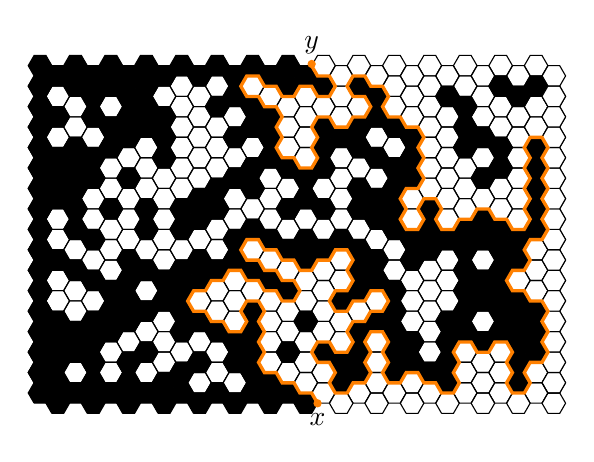
\begin{tikzpicture}
    \begin{scope}[scale=0.15]
      % seed 173
      \foreach \i in {-7,...,7} {
        \foreach \j in {-7,...,7} {
          \rand
          \draw [fill, fill opacity=\arabic{rand}] (\i*3, \j*1.732) -- ++(0:1) -- ++(60:1) -- ++(120:1) -- ++(180:1) -- ++(240:1) -- ++(300:1);
          \rand
          \draw [fill, fill opacity=\arabic{rand}] (\i*3 + 1.5, \j*1.732 - 0.866) -- ++(0:1) -- ++(60:1) -- ++(120:1) -- ++(180:1) -- ++(240:1) -- ++(300:1);
        }
      }
        \foreach \j in {-7,...,7} {
          \draw [fill] (-7*3, \j*1.732) -- ++(0:1) -- ++(60:1) -- ++(120:1) -- ++(180:1) -- ++(240:1) -- ++(300:1);
          \draw [fill=white] (7*3 + 1.5, \j*1.732 - 0.866) -- ++(0:1) -- ++(60:1) -- ++(120:1) -- ++(180:1) -- ++(240:1) -- ++(300:1);
        }

      \foreach \i in {-7,...,0} {
        \draw [fill] (\i*3, -8*1.732) -- ++(0:1) -- ++(60:1) -- ++(120:1) -- ++(180:1) -- ++(240:1) -- ++(300:1);
        \draw [fill] (\i*3 + 1.5, -8*1.732 - 0.866) -- ++(0:1) -- ++(60:1) -- ++(120:1) -- ++(180:1) -- ++(240:1) -- ++(300:1);
        \draw [fill] (\i*3, 8*1.732) -- ++(0:1) -- ++(60:1) -- ++(120:1) -- ++(180:1) -- ++(240:1) -- ++(300:1);
        \draw [fill] (\i*3 + 1.5, 8*1.732 - 0.866) -- ++(0:1) -- ++(60:1) -- ++(120:1) -- ++(180:1) -- ++(240:1) -- ++(300:1);
      }
      \foreach \i in {1,...,7} {
        \draw (\i*3, -8*1.732) -- ++(0:1) -- ++(60:1) -- ++(120:1) -- ++(180:1) -- ++(240:1) -- ++(300:1);
        \draw (\i*3 + 1.5, -8*1.732 - 0.866) -- ++(0:1) -- ++(60:1) -- ++(120:1) -- ++(180:1) -- ++(240:1) -- ++(300:1);
        \draw (\i*3, 8*1.732) -- ++(0:1) -- ++(60:1) -- ++(120:1) -- ++(180:1) -- ++(240:1) -- ++(300:1);
        \draw (\i*3 + 1.5, 8*1.732 - 0.866) -- ++(0:1) -- ++(60:1) -- ++(120:1) -- ++(180:1) -- ++(240:1) -- ++(300:1);
      }

      \node [circ, morange] at (3, -13.866) {};
      \node [below] at (3, -13.866) {$x$};
      \node [circ, morange] at (2.5, 14.866) {};
      \node [above] at (2.5, 14.866) {$y$};

      \draw [morange, very thick] (3, -13.866) -- ++(120:1) -- ++(180:1) -- ++(120:1) -- ++(180:1) -- ++(120:1) -- ++(180:1) -- ++(120:1) -- ++(60:1) -- ++(120:1) -- ++(60:1) -- ++(120:1) -- ++(60:1) -- ++(120:1) -- ++(180:1) -- ++(240:1) -- ++(300:1) -- ++(240:1) -- ++(180:1) -- ++(120:1) -- ++(180:1) -- ++(120:1) -- ++(180:1) -- ++(120:1) -- ++(60:1) -- ++(0:1) -- ++(60:1) -- ++(0:1) -- ++(60:1) -- ++(0:1) -- ++(300:1) -- ++(0:1) -- ++(300:1) -- ++(0:1) -- ++(300:1) -- ++(0:1) -- ++(60:1) -- ++(120:1) -- ++(180:1) -- ++(120:1) -- ++(180:1) -- ++(120:1) -- ++(180:1) -- ++(120:1) -- ++(60:1) -- ++(0:1) -- ++(300:1) -- ++(0:1) -- ++(300:1) -- ++(0:1) -- ++(300:1) -- ++(0:1) -- ++(60:1) -- ++(0:1) -- ++(60:1) -- ++(0:1) -- ++(300:1) -- ++(240:1) -- ++(300:1) -- ++(240:1) -- ++(180:1) -- ++(240:1) -- ++(300:1) -- ++(0:1) -- ++(60:1) -- ++(0:1) -- ++(60:1) -- ++(0:1) -- ++(300:1) -- ++(240:1) -- ++(180:1) -- ++(240:1) -- ++(180:1) -- ++(240:1) -- ++(300:1) -- ++(240:1) -- ++(180:1) -- ++(120:1) -- ++(180:1) -- ++(240:1) -- ++(300:1) -- ++(0:1) -- ++(300:1) -- ++(240:1) -- ++(300:1) -- ++(0:1) -- ++(60:1) -- ++(0:1) -- ++(60:1) -- ++(120:1) -- ++(60:1) -- ++(120:1) -- ++(60:1) -- ++(0:1) -- ++(300:1) -- ++(240:1) -- ++(300:1) -- ++(240:1) -- ++(300:1) -- ++(0:1) -- ++(60:1) -- ++(0:1) -- ++(300:1) -- ++(0:1) -- ++(300:1) -- ++(0:1) -- ++(60:1) -- ++(120:1) -- ++(60:1) -- ++(120:1) -- ++(60:1) -- ++(0:1) -- ++(300:1) -- ++(0:1) -- ++(60:1) -- ++(0:1) -- ++(300:1) -- ++(240:1) -- ++(300:1) -- ++(240:1) -- ++(300:1) -- ++(0:1) -- ++(60:1) -- ++(120:1) -- ++(60:1) -- ++(0:1) -- ++(60:1) -- ++(120:1) -- ++(60:1) -- ++(120:1) -- ++(60:1) -- ++(120:1) -- ++(180:1) -- ++(120:1) -- ++(180:1) -- ++(120:1) -- ++(60:1) -- ++(0:1) -- ++(60:1) -- ++(120:1) -- ++(60:1) -- ++(0:1) -- ++(60:1) -- ++(120:1) -- ++(60:1) -- ++(120:1) -- ++(60:1) -- ++(120:1) -- ++(60:1) -- ++(120:1) -- ++(60:1) -- ++(120:1) -- ++(180:1) -- ++(240:1) -- ++(300:1) -- ++(240:1) -- ++(300:1) -- ++(240:1) -- ++(300:1) -- ++(240:1) -- ++(300:1) -- ++(240:1) -- ++(180:1) -- ++(120:1) -- ++(180:1) -- ++(120:1) -- ++(180:1) -- ++(240:1) -- ++(180:1) -- ++(240:1) -- ++(180:1) -- ++(120:1) -- ++(60:1) -- ++(120:1) -- ++(180:1) -- ++(240:1) -- ++(300:1) -- ++(240:1) -- ++(180:1) -- ++(120:1) -- ++(60:1) -- ++(120:1) -- ++(60:1) -- ++(0:1) -- ++(60:1) -- ++(120:1) -- ++(60:1) -- ++(120:1) -- ++(60:1) -- ++(120:1) -- ++(180:1) -- ++(120:1) -- ++(180:1) -- ++(120:1) -- ++(60:1) -- ++(120:1) -- ++(180:1) -- ++(120:1) -- ++(180:1) -- ++(240:1) -- ++(300:1) -- ++(0:1) -- ++(300:1) -- ++(240:1) -- ++(180:1) -- ++(240:1) -- ++(180:1) -- ++(120:1) -- ++(180:1) -- ++(240:1) -- ++(300:1) -- ++(240:1) -- ++(300:1) -- ++(240:1) -- ++(180:1) -- ++(120:1) -- ++(180:1) -- ++(120:1) -- ++(60:1) -- ++(120:1) -- ++(60:1) -- ++(120:1) -- ++(180:1) -- ++(120:1) -- ++(180:1) -- ++(120:1) -- ++(60:1) -- ++(0:1) -- ++(300:1) -- ++(0:1) -- ++(300:1) -- ++(0:1) -- ++(60:1) -- ++(0:1) -- ++(300:1) -- ++(0:1) -- ++(60:1) -- ++(120:1) -- ++(180:1) -- ++(120:1);
    \end{scope}
  \end{tikzpicture}
\end{center}
Then there exists a unique interface $\gamma_\varepsilon$ that connects $x$ to $y$ with the property that the black hexagons on its left and white on its right. It was conjectured (and now proved by Smirnov) that the limit of the law of $\gamma_\varepsilon$ exists in distribution and is conformally invariant.

This means that if $\tilde{D}$ is another simply connected domain, and $\tilde{x}, \tilde{y} \in \partial \tilde{D}$ are distinct, then $\varphi: D \to \tilde{D}$ is a conformal transformation with $\varphi(x) = \tilde{x}$, $\varphi(y) = \tilde{y}$, then $\varphi(\gamma)$ is equal in distribution of the scaling limit of percolation in $\tilde{D}$ from $\tilde{x}$ to $\tilde{y}$.

Also, percolation also satisfies a natural Markov property: if we condition on $\gamma_\varepsilon$ up to a given time $t$, then the rest of $\gamma_\varepsilon$ is a percolation exploration in the remaining domain. The reason for this is very simple --- the path only determines the colours of the hexagons right next to it, and the others are still randomly distributed independently.

If we assume these two properties, then the limiting path $\gamma$ satisfies the conformal Markov property, and so must be an $\SLE_\kappa$. So the question is, what is $\kappa$?

To figure out this $\kappa$, we observe that the scaling limit of percolation has a locality property, and we will later see that $\SLE_6$ is the only SLE that satisfies this locality property.

To explain the locality property, fix a simply-connected domain $D$ in $\H$ (for simplicity), and assume that $0 \in \partial D$. Fixing a point $y \in \partial D$, we perform the percolation exploration as before. Then the resulting path would look exactly the same as if we performed percolation on $\H$ (with black boundary on $\R_{<0}$ and white boundary on $\R_{>0}$), up to the point we hit $\partial D \setminus \partial \H$. In other words, $\gamma$ doesn't feel the boundary conditions until it hits the boundary. This is known as \term{locality}.

It should then be true that the corresponding $\SLE_\kappa$ should have an analogous property. To be precise, we want to find a value of $\kappa$ so that the following is true: If $\gamma$ is an $\SLE_\kappa$ in $\H$ from $0$ to $\infty$, run up until it first hits $\partial D \setminus \partial \H$, then $\psi(\gamma)$ is a (stopped) $\SLE_\kappa$ in $\H$ from $0$ to $\infty$ where $\psi: D \to \H$ is a conformal transformation with $\psi(0) = 0$, $\psi(y) = \infty$. This is the \term{locality property}. We will show that locality holds precisely for $\kappa = 6$.

Suppose that $(A_t) \in \mathcal{A}$ has Loewner driving function $U_t$. We define
\[
  \tilde{A}_t = \psi(A_t).
\]
Then $\tilde{A}_t$ is a family of compact $\H$-hulls that are non-decreasing, locally growing, and $A_0 = \emptyset$. However, in general, this is not going to be parametrized by capacity. On the second example sheet, we show that this has half plane capacity
\[
  \tilde{a}(t) = \hcap(\tilde{A}_t) = \int_0^t \gamma(\psi_t'(U_s))^2\;\d s,
\]
which should be somewhat believable, given that $\hcap(rA) = r^2 \hcap(A)$.

$\tilde{A}_t$ has a ``driving function'' $\tilde{U}_t$ given by
\[
  \tilde{U}_t = \psi_t(U_t),\quad \psi_t = \tilde{g}_t \circ \psi \circ g_t^{-1},\quad g_t = g_{A_t}.
\]
We then have
\[
  \partial_t \tilde{g}_t (z) = \frac{\partial_t \tilde{a}_t}{\tilde{g}_t(z) - \tilde{U}_t},\quad \tilde{g}_0(z),
\]
To see this, simply recall that if $A_t$ is $\gamma([0, t])$ for a curve $\gamma$, then $U_t = g_t(\gamma(t))$.

To understand $\tilde{U}_t$, it is convenient to know something about $\psi_t$:
\begin{prop}
  The maps $(\psi_t)$ satisfy
  \[
    \partial_t \psi_t(z) = 2 \left(\frac{(\psi_t'(U_t))^2}{\psi_t(z) - \psi_t(U_t)} - \frac{\psi_t' (U_t)}{z - U_t}\right).
  \]
  In particular, at $z = U_t$, we have
  \[
    \partial_t \psi_t(U_t) = \lim_{z \to U_t} \partial_t \psi_t (z) = -3 \psi_t''(U_t).
  \]
\end{prop}

\begin{proof}
  These are essentially basic calculus computations.
\end{proof}

To get Loewner's equation in the right shape, we perform a time change
\[
  \sigma(t) = \inf \left\{u \geq 0: \int_0^u (\psi_s'(U_s))^2 \;\d s = t\right\}.
\]
Then we have
\[
  \partial_t \tilde{g}_{\sigma(t)} (z) = \frac{2}{\tilde{g}_{\sigma(t)} - \tilde{U}_{\sigma(t)}},\quad \tilde{g}_0(z) = z.
\]

It then remains to try to understand $\d \tilde{U}_{\sigma(t)}$. Note that so far what we said works for general $U_t$. If we put $U_t = \sqrt{\kappa} B_t$, where $B$ is a standard Brownian motion, then It\^o's formula tells us before the time change, we have
\begin{align*}
  \d \tilde{U}_t &= \d \psi_t(U_t) \\
  &= \left(\partial_t \psi_t(U_t) + \frac{\kappa}{2} \psi_t'' (U_t)\right)\;\d t + \sqrt{\kappa} \psi_t'(U_t)\;\d B_t\\
  &= \frac{\kappa - 6}{2} \psi_t''(U_t) \;\d t + \sqrt{\kappa} \psi_t'(U_t)\;\d B_t.
\end{align*}
After the time change, we get
\[
  \d \tilde{U}_{\sigma(t)} = \frac{\kappa - 6}{2} \frac{\psi_{\sigma(t)}'' (U_{\sigma(t)})}{\psi_{\sigma(t)}' (U_{\sigma(t)})^2} \;\d t + \sqrt{\kappa} \;\d \tilde{B}_t,
\]
where
\[
  \tilde{B}_t = \int_0^{\sigma(t)} \psi_s'(U_s) \;\d B_s
\]
is a standard Brownian motion by the L\'evy characterization and the definition of $\sigma(t)$.

The point is that when $\kappa = 6$, the drift term goes away, and so
\[
  \tilde{U}_{\sigma(t)} = \sqrt{6} \tilde{B}_t.
\]
So $(\tilde{A}_{\sigma(t)})$ is an $\SLE_6$. Thus, we have proved that
\begin{thm}
  If $\gamma$ is an $\SLE_\kappa$, then $\psi(\gamma)$ is an $\SLE_\kappa$ up until hitting $\psi(\partial D \setminus \partial \H)$ if and only if $\kappa = 6$.
\end{thm}

So $\kappa = 6$ is the only possible $\SLE_\kappa$ which could be the limit of percolation.

\section{Scaling limit of self-avoiding walks}\label{sec:saw}
We next think about self-avoiding walk (SAW).

\begin{defi}[Self-avoiding walk]\index{self-avoiding walk}
  Let $G = (V, E)$ be a graph with uniformly bounded degree, and pick $x \in V$ and $n \in \N$. The self-avoiding in $G$ starting from $x$ of length $n$ is the uniform measure on \emph{simple} paths in $G$ starting from $x$ of length $n$.
\end{defi}
Self-avoiding walk tends to be difficult to understand, since they usually don't have the Markov property. However, in the scaling limit, it tends to be more well-behaved. Restricting to the case of $G = \Z^d$, it has been shown that for $d \geq 5$, the scaling limit is just Brownian motion (Hara and Slade).

In $d = 4$, the same is conjectured to be true. In $d = 3$, there is no conjecture for the continuous object which should describe its scaling limit. In this course, we are only interested in $d = 2$. In this case, the self-avoiding walk is conjectured to converge to $\SLE_{8/3}$ (Lawler--Schramm--Werner).

In percolation, the property that allowed us to conclude that the scaling limit was $\SLE_6$ is the locality property. In self-avoiding walks, the special property is \emph{restriction}. This is a very simple concept --- if $G' = (V', E')$ is a subgraph of $G$ with $x \in V'$, then the self-avoiding walk on $G$ conditioned to stay in $G'$ is a self-avoiding walk on $G'$. Indeed, uniform measures always restricts to the uniform measure on a smaller subset. It turns out $\SLE_{8/3}$ is the only $\SLE$ which satisfies a continuum version of restriction. We will only show one direction, namely that $\SLE_{8/3}$ satisfies the restriction property, but the other direction is also known.

\subsubsection*{Brownian excursion}
When studying the restriction property, we will encounter another type of process, known as \emph{Brownian excursion}. Fix a simply connected domain $D \subseteq \C$ and points $x, y \in \partial D$ distinct. Then roughly speaking, a Brownian excursion is a Brownian motion starting at $x$ conditioned to leave $D$ at $\partial D$. Of course, we cannot interpret these words literally, since we want to condition on a zero probability event.

To make this rigorous, we first use conformal invariance to say we only have to define this for $\H$ with $x = 0$, $y = \infty$.

To construct it in $\H$, we start with a complex Brownian motion $B = B^1 + i B^2$, with $B^1_0 = 0$ and $B_0^2 = \varepsilon > 0$. We then condition $B$ on the event that $B^2$ hits $R \gg 0$ before hitting $0$. This is a positive probability event. We then take limits $R \to \infty$ and $\varepsilon \to 0$. On the second example sheet, we will show that this makes sense, and the result is called \term{Brownian excursion}.

It turns out the limiting object is pretty simple. It is given by
\[
  \hat{B} = (\hat{B}^1, \hat{B}^2)
\]
where $\hat{B}^1$ is a standard Brownian motion and $\hat{B}^2 \sim \BES^3$, and the two are independent.

The key property about Brownian excursion we will need is the following:
\begin{prop}
  Suppose $A$ be a compact $\H$-hull and $g_A$ is as usual. If $x \in \R \setminus A$, then
  \[
    \P_x[\hat{B}[0, \infty) \cap A = \emptyset] = g_A'(x).
  \]
\end{prop}

\begin{proof}
  This is a straightforward computation. Take $z = x + i \varepsilon$ with $\varepsilon > 0$, and let $B_t$ be a Brownian motion. Define
  \[
    \sigma_R = \inf \{t \geq 0: \im(B_t) = R\}.
  \]
  Then the desired probability is
  \[
    \lim_{\varepsilon \to 0} \lim_{R \to \infty} \P_z [B[0, \sigma_R] \cap A = \emptyset \mid B[0, \sigma_R] \cap \R = \emptyset].
  \]
  By Bayes' theorem, this is equal to
  \[
    \lim_{\varepsilon \to 0}\lim_{R \to \infty} \frac{\P_z[B[0, \sigma_R] \cap (A \cup \R) = \emptyset]}{\P[B[0, \sigma_R] \cap \R = \emptyset]}.
  \]
  We understand the numerator and denominator separately. The gambler's ruin estimate says the denominator is just $\varepsilon/R$, and to bound the numerator, recall that for $z \in \H \setminus A$, we have
  \[
    |g_A(z) - z| \leq 3 \rad(A).
  \]
  Thus, using conformal invariance, we can bound
  \begin{multline*}
    \P_{g_A(z)} [B[0, \sigma_{R + 3\rad(A)}] \cap \R = \emptyset] \leq \P_z[B[0, \sigma_R] \cap (A \cup \R) = \emptyset]\\
    \leq \P_{g_A(z)}[B[0, \sigma_{R - 3 \rad(A)}] \cap \R = \emptyset].
  \end{multline*}
  So we get
  \[
    \frac{\im(g_A(z))}{R+ 3 \rad(A)} \leq \text{numerator} \leq \frac{\im(g_A(z))}{R - 3 \rad(Z)}.
  \]
  Combining, we find that the desired probability is
  \[
    \lim_{\varepsilon \to 0} \frac{\im(g_A(x + i \varepsilon))}{\varepsilon} = g_A'(x).\qedhere
  \]
\end{proof}

\subsubsection*{The restriction property}
We now return to understanding the restriction property. We assume that $\kappa \leq 4$, since this is the range of $\kappa$-values so that $\SLE_\kappa$ is simple.

Recall that $\mathcal{Q}$ is the set of all compact $\H$-hulls. We define
\begin{align*}
  \mathcal{Q}_+ &= \{A \in \mathcal{Q} : \bar{A} \cap (-\infty, 0] = \emptyset\}\\\
  \mathcal{Q}_- &= \{A \in \mathcal{Q} : \bar{A} \cap [0, \infty) = \emptyset\}
\end{align*}
For $A \in \mathcal{Q}_{\pm} = \mathcal{Q}_+ \cup \mathcal{Q}_-$, we define $\psi_A: \H \to A \to \H$ by
\[
  \psi_A(z) = g_A(z) - g_A(0).
\]
This is the version of $g_A$ that fixes $0$, which is what we need. This is the unique conformal transformation with
\[
  \psi_A(0) = 0,\quad \lim_{z \to \infty} \frac{\psi_A(z)}{z} = 1.
\]

We will need the following fact about SLE:
\begin{fact}
  $\SLE_\kappa$ is transient, i.e.\ if $\gamma$ is an $\SLE_\kappa$ in $\H$ from $0$ to $\infty$, then
  \[
    \lim_{t \to \infty} \gamma(t) = \infty\text{ almost surely}.
  \]
\end{fact}
This is not very difficult to prove, but the proof is uninteresting and we have limited time. Since $\SLE_\kappa$ is simple for $\kappa \leq 4$ and is also transient, it follows that for all $A \in \mathcal{Q}_{\pm}$,
\[
  0 < \P[\gamma[0, \infty) \cap A = \emptyset] < 1.
\]
This is useful because we want to condition on this event. Write
\[
  V_A = \{\gamma[0, \infty) \cap A = \emptyset\}.
\]
\begin{defi}[Restriction property]\index{restriction property}
  We say an $\SLE_\kappa$ satisfies the restriction property if whenever $\gamma$ is an $\SLE_\kappa$, for any $A \in \mathcal{Q}_{\pm}$, the law of $\psi_A(\gamma)$ conditional on $V_A$ is that of an $\SLE_\kappa$ curve (for the same $\kappa$).
\end{defi}

Observe that the law of $\gamma$ is determined by the probabilities $A \mapsto \P[V_A]$ for all $A \in \mathcal{Q}_{\pm}$.

\begin{lemma}
  Suppose there exists $\alpha > 0$ so that
  \[
    \P[V_A] = (\psi_A'(0))^\alpha
  \]
  for all $A \in \mathcal{Q}_{\pm}$, then $\SLE_\kappa$ satisfies restriction.
\end{lemma}

\begin{proof}
  Suppose the assertion in the lemma is true. Suppose that $A, B \in \mathcal{Q}_{\pm}$. Then we have that
  \begin{align*}
    \P[\psi_A(\gamma[0, \infty)) \cap B = \emptyset \mid V_A] &= \frac{\P[\gamma[0, \infty) \cap (\psi_A^{-1}(B) \cup A) = \emptyset]}{\P[\gamma[0, \infty) \cap A = \emptyset]}\\
    &= \frac{(\psi_{(\psi_A^{-1}(B) \cup A)}'(0))^\alpha}{(\psi_A'(0))^\alpha}\\
    &= \frac{(\psi_B'(0))^\alpha (\psi_A'(0))^\alpha}{(\psi_A'(0))^\alpha}\\
    &= (\psi_B'(0))^\alpha\\
    &= \P[V_B],
  \end{align*}
  where we used that
  \[
    \psi_{\psi_A^{-1}(B) \cup A} = \psi_B \circ \psi_A.
  \]
  So the law of $\psi_A(\gamma)$ given $V_A$ is the law of $\gamma$.
\end{proof}

We now have to show that $\SLE_{8/3}$ satisfies the condition in the lemma. Let $\mathcal{F}_t$ be the filtration of $U_t = \sqrt{\kappa} B_t$. Then
\[
  \tilde{M}_t = \P[V_A \mid \mathcal{F}_t]
\]
is a bounded martingale with $\tilde{M}_0 = \P[V_A]$. Also,
\[
  \tilde{M}_t \to \mathbf{1}_{V_A}
\]
by the martingale convergence theorem. Also, if we define the stopping time
\[
  \tau = \inf \{t \geq 0: \gamma(t) \in A\},
\]
then we get
\[
  \tilde{M}_T = \P[V_A \mid \mathcal{F}_t] = \P[V_A \mid \mathcal{F}_t] \mathbf{1}_{\{t < \tau\}} = \P[V_{g_t(A) - g_t(0)}] \mathbf{1}_{\{t < \tau\}}
\]
by the conformal Markov property.

Observe that if $M_t$ is another bounded $\mathcal{F}_t$-martingale with the property that $M_t \to \mathbf{1}_{V_A}$ as $t \to \infty$, then $M_t = \tilde{M}_t$ for all $t \geq 0$, since
\[
  M_t = \E[\mathbf{1}_{V_A} \mid \mathcal{F}_t] = \tilde{M}_t.
\]
Given what we were aiming for, we consider
\[
  M_t = (\psi_{g_t(A) - g_t(0)}'(0))^\alpha \mathbf{1}_{\{t < \tau\}}
\]
\begin{lemma}
  $M_{t \wedge \tau}$ is a continuous martingale if
  \[
    \kappa = \frac{8}{3},\quad \alpha = \frac{5}{8}.
  \]
\end{lemma}
These numbers are just what comes out when we do the computations.

\begin{proof}
  Recall that we showed that $g'_A$ is a probability involving Brownian excursion, and in particular is bounded in $[0, 1]$. So the same is true for $\psi'_A$, and hence $M_{t \wedge \tau}$. So it suffices to show that $M_{t \wedge \tau}$ is a continuous local martingale. Observe that
  \[
    M_{t \wedge \tau} = (\psi_{g_{t \wedge \tau}(A) - g_{t \wedge \tau}(0)}'(0))^\alpha
  \]
  So if we define
  \[
    N_t = (\psi_{g_t(A) - g_t(0)}'(0))^\alpha,
  \]
  then it suffices to show that $N_t$ is a continuous local martingale by optional stopping. We write
  \[
    \psi_t = \tilde{g}_t \circ \psi_A \circ g_t^{-1},
  \]
  where $\tilde{g}_t = g_{\psi_A(\gamma(0, t])}$. We then have
  \[
    N_t = (\psi_t'(U_t))^\alpha.
  \]
  In the example sheet, we show that
  \[
    \partial_t \psi_t' (U_t) = \frac{\psi_t''(U_t)^2}{2\psi_t'(U_t)} - \frac{4}{3} \psi_t'''(U_t).
  \]
  By It\^o's formula, we get
  \begin{multline*}
    \d N_t = \alpha N_t \left[\frac{(\alpha - 1)\kappa + 1}{2} \frac{\psi_t''(U_t)^2}{\psi_t'(U_t)^2} + \left(\frac{\kappa}{2} - \frac{4}{3}\right) \frac{\psi_t'''(U_t)}{\psi_t'(U_t)}\right]\;\d t \\
    + \alpha N_t \frac{\psi_t''(U_t)}{\psi_t'(U_t)} \cdot \sqrt{\kappa} \;\d B_t.
  \end{multline*}
  Picking $\kappa = \frac{8}{3}$ ensures the second $\d t$ term vanishes, and then setting $\alpha = \frac{5}{8}$ kills the first $\d t$ term as well, and we are done.
\end{proof}

We next want to establish that $M_t \to \mathbf{1}_{V_A}$ as $t \to \infty$.

Recall that $M_t$ is the probability that a Brownian excursion on $\H \setminus \gamma[0, t]$ from $\gamma(t)$ to infinity does not hit $A$. So we would expect this to be true, since on $V_A$, as $t$ increases, the tip of the SLE gets further and further away from $A$, and so it is difficult for a Brownian excursion to hit $A$; conversely on $V_A^C$, it eventually gets to $A$, and then we are dead.

By scaling, we can assume that
\[
  \sup \{\im(\omega): \omega \in A\} = 1.
\]
It is convenient to define the stopping times
\[
  \sigma(r) = \inf \{t \geq 0 : \im(\gamma(t)) = r\}.
\]
Note that $\sigma_r < \infty$ almost surely for all $r > 0$ since $\SLE_{8/3}$ is transient.

\begin{lemma}
  $M_{t \wedge \tau} \to 1$ on $V_A$ as $t \to \infty$.
\end{lemma}

\begin{proof}
  Let $\hat{B}$ be a Brownian excursion in $\H \setminus \gamma[0, \sigma_r]$ from $\gamma(\sigma_r)$ to $\infty$. Let $B$ be a complex Brownian motion, and
  \[
    \tau_R = \inf\{t \geq 0: \im(B_t) = R\},\quad z = \gamma(\sigma_r) + i\varepsilon.
  \]
  Then the probability that $\hat{B}$ hits $A$ is
  \[
    1 - \psi_{\sigma_r}'(U_{\sigma_r}) = \lim_{\varepsilon \to 0} \lim_{R \to \infty} \frac{\P_z [B[0, \tau_R] \subseteq \H \setminus \gamma[0, \sigma_r], B[0, \tau_R] \cap A \not= \emptyset]}{\P_z[B[0, \tau_R] \subseteq \H \setminus \gamma[0, \sigma_r]]},\tag{$*$}
  \]
  We will show that this expression is $\leq C r^{-1/2}$ for some constant $C > 0$. Then we know that $M_{\sigma_r \wedge \tau} \to 1$ as $r \to \infty$ on $V_A$. This is convergence along a subsequence, but since we already know that $M_{t \wedge \tau}$ converges this is enough.

  We first tackle the denominator, which we want to bound from below. The idea is to bound the probability that the Brownian motion reaches the lime $\im(z) = r + 1$ without hitting $\R \cup \gamma[0, \sigma_r]$. Afterwards, the gambler's ruin estimate tells us the probability of reaching $\im(z) = R$ without going below the $\im(z) = r$ line is $\frac{1}{R - r}$.

  In fact, we shall consider the box $S = [-1, 1]^2 + \gamma(\sigma_r)$ of side length $2$ centered at $\gamma(\sigma_r)$. Let $\eta$ be the first time $B$ leaves $S$, and we want this to leave via the top edge $\ell$. By symmetry, if we started right at $\gamma(\sigma_r)$, then the probability of leaving at $\ell$ is exactly $\frac{1}{4}$. Thus, if we are at $z = \gamma(\sigma_r) + i\varepsilon$, then the probability of leaving via $\ell$ is $> \frac{1}{4}$.

  What we would want to show is that
  \[
    \P_z[B(\eta) \in \ell \mid B[0, \eta] \cap \gamma[0, \sigma_r] = \emptyset] > \frac{1}{4}.\tag{$\dagger$}
  \]
  We then have the estimate
  \[
    \text{denominator} \geq \frac{1}{4}\cdot \P_z[B[0, \eta] \cap \gamma[0, \sigma_r] = \emptyset] \cdot \frac{1}{R - r}.
  \]
  Intuitively, $(\dagger)$ must be true, because $\gamma[0, \sigma_r]$ lies below $\im(z) = r$, and so if $B[0, \eta]$ doesn't hit $\gamma[0, \sigma_r]$, then it is more likely to go upwards. To make this rigorous, we write
  \begin{align*}
    \frac{1}{4} &< \P_z[B(\eta) \in \ell]\\
    &= \P_z[B(\eta) \in \ell \mid B[0, \eta] \cap \gamma[0, \sigma_r] = \emptyset]\; \P[B[0, \eta] \cap \gamma[0, \sigma_r] = \emptyset]\\
    &\,+\P_z[B(\eta) \in \ell \mid B[0, \eta] \cap \gamma[0, \sigma_r] \not= \emptyset]\;\P[ B[0, \eta] \cap \gamma[0, \sigma_r] \not= \emptyset]
  \end{align*}
  To prove $(\dagger)$, it suffices to observe that the first factor of the second term is $\leq \frac{1}{4}$, which follows from the strong Markov property, since $\P_w[B(\eta) \in \ell] \leq \frac{1}{4}$ whenever $\im(w)\leq r$, which in particular is the case when $w \in \gamma[0, \sigma_r]$.

  To bound the numerator, we use the strong Markov property and the Beurling estimate to get
  \[
    \P_z[B\text{ hits $A$ without hitting }\R \cup \gamma[0, \sigma_r]] \leq \P_z[B[0, \eta] \cap \gamma[0, \sigma_r]] \cdot C r^{-1/2}.
  \]
  Combining, we know the numerator in $(*)$ is
  \[
    \leq \frac{1}{R} C \cdot r^{-1/2} \cdot \P[B[0, \eta] \cap \gamma[0, \sigma_r] = \emptyset].
  \]
  These together give the result.
\end{proof}

\begin{lemma}
  $M_{t \wedge \tau} \to 0$ as $t \to \infty$ on $V_A^c$.
\end{lemma}

This has a ``shorter'' proof, because we outsource a lot of the work to the second example sheet.
\begin{proof}
  By the example sheet, we may assume that $A$ is bounded by a smooth, simple curve $\beta: (0, 1) \to \H$.

  Note that $\gamma(\tau) = \beta(s)$ for some $s \in (0, 1)$. We need to show that
  \[
    \lim_{t \to \tau} \psi_t'(U_t) = 0.
  \]
  For $m \in \N$, let
  \[
    t_m = \inf \left\{t \geq 0 : |\gamma(t) - \beta(s)| = \frac{1}{m}\right\}
  \]
  Since $\beta$ is smooth, there exists $\delta > 0$ so that
  \[
    \ell = [\beta (s), \beta(s) + \delta \mathbf{n}] \subseteq A,
  \]
  where $\mathbf{n}$ is the unit inward pointing normal at $\beta(s)$. Let
  \[
    L_t = g_t(\ell) - U_t.
  \]
  Note that a Brownian motion starting from a point on $\ell$ has a uniformly positive chance of exiting $\H \setminus \gamma[0 ,t_m]$ on the left side of $\gamma[0, t_m]$ and on the right side as well.

  On the second example sheet, we see that this implies that
  \[
    L_{t_m} \subseteq \{w : \im (w) \geq a |\Re(w)|\}
  \]
  for some $a > 0$, using the conformal invariance of Brownian motion. Intuitively, this is because after applying $g_t - U_t$, we have uniformly positive probability of exiting via the positive or real axis, and so we cannot be too far away in one directionn.

  Again by the second example sheet, the Brownian excursion in $\H$ from $0$ to $\infty$ hits $L_{t_m}$ with probability $\to 1$ as $m \to \infty$.
\end{proof}

We thus conclude
\begin{thm}
  $\SLE_{8/3}$ satisfies the restriction property. Moreover, if $\gamma \sim \SLE_{8/3}$, then
  \[
    \P[\gamma[0, \infty) \cap A = \emptyset] = (\psi_A'(0))^{5/8}.\qedhere
  \]
\end{thm}

There is a rather surprising consequence of this computation. Take $\gamma_1, \ldots, \gamma_8$ to be independent $\SLE_{8/3}$'s. Then we have
\[
  \P[\gamma_j[0, \infty) \cap A = \emptyset\text{ for all }j] = (\psi_A'(0))^5.
\]
Note that this is the same as the probability that the hull of $\gamma_1, \ldots, \gamma_8$ des not intersect $A$, where the hull is the union of the $\gamma_j$'s together with the bounded components of $\H \setminus \bigcup_j \gamma_j$.

In the same manner, if $\hat{B}_1, \ldots, \hat{B}_5$ are independent Brownian excursions, then
\[
  \P[\hat{B}_j[0, \infty) \cap A = \emptyset\text{ for all }j] = (\psi_A'(0))^5.
\]
Thus, the hull of $\gamma_1, \ldots, \gamma_8$ has the same distribution as the hull of $\hat{B}_1, \ldots, \hat{B}_5$.

Moreover, if we take a boundary point of the hull of, say, $\gamma_1, \ldots, \gamma_8$, then we would expect it to belong to just one of the $\SLE_{8/3}$'s. So the boundary of the hull of $\gamma_1, \ldots, \gamma_8$ looks locally like an $\SLE_{8/3}$, and the same can be said for the hull fo $\hat{B}_1, \ldots, \hat{B}_5$. Thus, we conclude that the boundary of a Brownian excursion looks ``locally'' like $\SLE_{8/3}$.

\section{The Gaussian free field}\label{sec:gff}
We end by discussing the Gaussian free field, which we can think of as a two-dimensional analogue of Brownian motion, i.e.\ a random surface. We will show that the level curves of the Gaussian free field are $\SLE_4$s.

To define the Gaussian free field, we have to do some analysis.
\begin{notation}\leavevmode
  \begin{itemize}
    \item $C^\infty$ is the space of infinitely differentiable functions on $\C$
    \item $C_0^\infty$ is the space of functions in $C^\infty$ with compact support.
    \item If $D$ is a domain, $C_0^\infty(D)$ is the functions in $C_0^\infty$ supported in $D$.
  \end{itemize}
\end{notation}

\begin{defi}[Dirichlet inner product]\index{Dirichlet inner product}
  Let $f, g \in C_0^\infty$. The \emph{Dirichlet inner product} of $f, g$ is
  \[
    (f, g)_\nabla = \frac{1}{2\pi}\int \nabla f(x) \cdot \nabla g(x)\;\d x.
  \]
\end{defi}
This defines an inner product function on $C_0^\infty$. If $D \subseteq \C$ is a non-trivial simply-connected domain, i.e.\ not $\emptyset$ or $\C$, we can define

\begin{defi}[$H_0^1(D)$]\index{$H_0^1(D)$}
  We write $H_0^1(D)$ for the Hilbert space completion of $C_0^\infty(D)$ with respect to $(\ph, \ph)_{\nabla}$.
\end{defi}
Elements of $H_0^1(D)$ can be thought of as functions well-defined up to a null set. These functions need not be continuous (i.e.\ need not have a continuous representatives), and in particular need not be genuinely differentiable, but they have ``weak derivatives''.

We will need the following key properties of $H_0^1(D)$:
\begin{prop}\leavevmode
  \begin{enumerate}
    \item Conformal invariance: Suppose $\varphi: D \to \tilde{D}$ is a conformal transformation, and $f, g \in C_0^\infty(D)$. Then
      \[
        (f, g)_\nabla = (f \circ \varphi^{-1}, g \circ \varphi^{-1})_\nabla
      \]
      In other words, the Dirichlet inner product is conformally invariant.

      In other words, $\varphi^*: H_0^1(D) \to H_0^1(\tilde{D})$ given by $f \mapsto f \circ \varphi^{-1}$ is an isomorphism of Hilbert spaces.
    \item Inclusion: Suppose $U \subseteq D$ is open. If $f \in C_0^\infty(U)$, then $f \in C_0^\infty(D)$. Therefore the inclusion map $i: H_0^1(U) \to H_0^1(D)$ is well-defined and associates $H_0^1(U)$ with a subspace of $H_0^1(D)$. We write the image as $H_{\mathrm{supp}}(U)$.
    \item Orthogonal decomposition: If $U \subseteq D$, let
      \[
        H_{\mathrm{harm}}(U) = \{f \in H_0^1(D): f\text{ is harmonic on }U\}.
      \]
      Then
      \[
        H_0^1(D) = H_{\mathrm{supp}}(U) \oplus H_{\mathrm{harm}}(U)
      \]
      is an orthogonal decomposition of $H_0^1(D)$. This is going to translate to a Markov property of the Gaussian free field.
  \end{enumerate}
\end{prop}

\begin{proof}
  Conformal invariance is a routine calculation, and inclusion does not require proof. To prove orthogonality, suppose $f \in H_{\mathrm{supp}}(U)$ and $g \in H_{\mathrm{harm}}(U)$. Then
  \[
    (f, g) = \frac{1}{2\pi} \int \nabla f(x) \cdot \nabla g(x) \;\d x =- \frac{1}{2\pi} \int f(x) \Delta g(x)\;\d x = 0.
  \]
  since $f$ is supported on $U$ and $\Delta g$ is supported outside of $U$.

  To prove that they span, suppose $f \in H_0^1(D)$, and $f_0$ the orthogonal projection of $f$ onto $H_{\mathrm{supp}}(U)$. Let $g_0 = f - f_0$. We want to show that $g_0$ is harmonic. It would be a straightforward manipulation if we can take $\Delta$, but there is no guarantee that $f_0$ is smooth.

  We shall show that $g_0$ is weakly harmonic, and then it is a standard analysis result (which is also on the example sheet) that $g_0$ is in fact genuinely harmonic.

  Suppose $\varphi \in C_0^\infty(U)$. Then since $g_0 \perp H_{\mathrm{supp}}(U)$, we have
  \[
    0 = (g_0, \varphi) = \frac{1}{2\pi} \int \nabla g_0(x) \cdot \nabla \varphi(x)\;\d x = - \frac{1}{2\pi} \int g_0(x) \Delta \varphi(x)\;\d x.
  \]
  This implies $g_0$ is $C^\infty$ on $U$ and harmonic.
\end{proof}

We will define the Gaussian free field to be a Gaussian taking values in $H_0^1$. To make this precise, we first understand how Gaussian random variables on $\R^n$ work.

Observe that if $\alpha_1, \ldots, \alpha_n$ are iid $N(0, 1)$ variables, and $e_1, \ldots, e_n$ is a standard basis of $R^n$, then
\[
  h = \alpha_1 e_1 + \cdots + \alpha_n e_n
\]
is a standard $n$-dimensional Gaussian random variable.

If $x = \sum x_j e_j \in \R^n$, then
\[
  (h, x) = \sum_{j = 1}^n \alpha_j x_j \sim N(0, \|x\|).
\]
Moreover, if $x, y \in \R^n$, then $(h, x)$ and $(h, y)$ are jointly Gaussian with covariance $(x, y)$.

Thus, we can associate with $h$ a \emph{family} of Gaussian random variables $(h, x)$ indexed by $x \in \R^n$ with mean zero and covariance given by the inner product on $\R^n$. This is an example of a \term{Gaussian Hilbert space}.

We now just do the same for the infinite-dimensional vector space $H_0^1(D)$. One can show that this is separable, and so we can pick an orthonormal basis $(f_n)$. Then the Gaussian free field $h$ on $D$ is defined by
\[
  h = \sum_{j = 1}^\infty \alpha_j f_j,
\]
where the $\alpha_j$'s are iid $N(0, 1)$ random variables. Thus, if $f \in H_0^1(D)$, then
\[
  (h, f)_\nabla \sim N(0, \|f\|_\nabla^2).
\]
More generally, if $f, g \in H_0^1(D)$, then $(h, f)_\nabla$ and $(h, g)_\nabla$ are jointly Gaussian with covariance $(f, g)_\nabla$. Thus, the Gaussian free field is a family of Gaussian variables $(H, f)_\nabla$ indexed by $f \in H_0^1(D)$ with mean zero and covariance $(\ph, \ph)_\nabla$.

We can't actually quite make this definition, because the sum $h = \sum_{j = 1}^\infty \alpha_j f_j$ does not converge. So $h$ is not really a function, but a distribution. However, this difference usually does not matter.

We can translate the properties of $H_0^1$ into analogous properties of the Gaussian free field.
\begin{prop}\leavevmode
  \begin{enumerate}
    \item If $\varphi: D \to \tilde{D}$ is a conformal transformation and $h$ is a Gaussian free field on $D$, then $h \circ \varphi^{-1}$ is a Gaussian free field on $\tilde{D}$.
    \item Markov property: If $U \subseteq D$ is open, then we can write $h = h_1 + h_2$ with $h_1$ and $h_2$ independent where $h_1$ is a Gaussian free field on $U_1$ and $h_2$ is harmonic on $U$.
  \end{enumerate}
\end{prop}

\begin{proof}\leavevmode
  \begin{enumerate}
    \item Clear.
    \item Take $h_1$ to be the projection onto $H_{\mathrm{supp}}(U)$. This works since we can take the orthonormal basis $(f_n)$ to be the union of an orthonormal basis of $H_{\mathrm{supp}}(U)$ plus an orthonormal basis of $H_{\mathrm{harm}}(U)$.\qedhere
  \end{enumerate}
\end{proof}

Often, we would rather think about the $L^2$ inner product of $h$ with something else. Observe that integration by parts tells us
\[
  (h, f)_\nabla = \frac{-1}{2\pi} (h, \Delta f)_{L^2}.
\]
Thus, we would be happy if we can invert $\Delta$, which we can by IB methods. Recall that
\[
  \Delta (- \log|x - y|) = -2\pi \delta(y - x),
\]
where $\Delta$ acts on $x$, and so $-\log|x - y|$ is a Green's function for $\Delta$. Given a domain $D$, we wish to obtain a version of the Green's function that vanishes on the boundary. To do so, we solve $\Delta \tilde{G}_x = 0$ on $D$ with the boundary conditions
\[
  \tilde{G}_x(y) = -\log|x - y|\text{ if }y \in \partial D.
\]
We can then set
\[
  G(x, y) = - \log |x - y| - \tilde{G}_x(y).
\]
With this definition, we can define
\[
  \Delta^{-1} \varphi(x) = -\frac{1}{2\pi} \int G(x, y) \varphi(y)\;\d y.
\]
Then $\Delta \Delta^{-1} \varphi(x) = \varphi(x)$, and so
\[
  (h, \varphi) \equiv (h, \varphi)_{L^2} = -2\pi (h, \Delta^{-1} \varphi)_\nabla.
\]
Then $(h, \varphi)$ is a mean-zero Gaussian with variance
\begin{align*}
  (2\pi)^2 \|\Delta^{-1} \varphi\|_{\nabla}^2 &= (2\pi)^2 (\Delta^{-1}\varphi, \Delta^{-1}\varphi)_{\nabla} \\
  &= - 2\pi (\Delta^{-1} \varphi, \Delta \Delta^{-1}\varphi)\\
  &= (-2\pi \Delta^{-1} \varphi, \varphi)\\
  &= \iint \varphi(x) G(x, y) \varphi(y)\;\d x\;\d y.
\end{align*}
More generally, if $\varphi, \psi \in C_0^\infty(D)$, then
\[
  \cov( (h, \varphi), (h, \psi)) = \iint \varphi(x) G(x, y) \psi(y)\;\d x\;\d y.
\]

On the upper half plane, we have a very explicit Green's function
\[
  G(x, y) = G_\H(x, y) = -\log |x - y| + \log |x - \bar{y}|.
\]
It is not hard to show that the Green's function is in fact conformally invariant:
\begin{prop}
  Let $D, \tilde{D}$ be domains in $\C$ and $\varphi$ is a conformal transformation $D \to \tilde{D}$. Then $G_D(x, y) = G_{\tilde{D}}(\varphi(x), \varphi(y))$.\fakeqed
\end{prop}
One way to prove this is to use the conformal invariance of Brownian motion, but a direct computation suffices as well.

Schramm and Sheffield showed that the level sets of $h$, i.e.\ $\{x : h(x) = 0\}$ are $\SLE_4$'s. It takes some work to make this precise, since $h$ is not a genuine function, but the formal statement is as follows:
\begin{thm}[Schramm--Sheffield]
  Let $\lambda = \frac{\pi}{2}$. Let $\gamma \sim \SLE_4$ in $\H$ from $0$ to $\infty$. Let $g_t$ its Loewner evolution with driving function $U_t = \sqrt{\kappa} B_t = 2 B_t$, and set $f_t = g_t - U_t$. Fix $W \subseteq \H$ open and let
  \[
    \tau = \inf \{t \geq 0: \gamma(t) \in W\}.
  \]
  Let $h$ be a Gaussian free field on $\H$, $\lambda > 0$, and $\mathscr{h}$ be the unique harmonic function on $\H$ with boundary values $\lambda$ on $\R_{>0}$ and $-\lambda$ on $\R_{<0}$. Explicitly, it is given by
  \[
    \mathscr{h} = \lambda - \frac{2\lambda}{\pi} \arg(\ph).
  \]
  Then
  \[
    h + \mathscr{h} \overset{d}{=} (h + \mathscr{h}) \circ f_{t \wedge \tau},
  \]
  where both sides are restricted to $W$.
\end{thm}
A few words should be said about why we should think of this as saying the level curves of $h$ are $\SLE_4$'s. First, observe that since $\mathscr{h}$ is harmonic, adding $\mathscr{h}$ to $h$ doesn't change how $h$ pairs with other functions in $H_0^1(\H)$. All it does is to change the boundary conditions of $h$. So we should think of $h + \mathscr{h}$ as a version of the Gaussian free field with boundary conditions
\[
  (h + \mathscr{h})(x) = \sgn(x) \lambda.
\]
It is comforting to know the fact that the boundary conditions of $h$ is well-defined as an element of $L^2$.

Similarly, $(h + \mathscr{h}) \circ f_{t \wedge \tau}$ is a Gaussian free field with the boundary condition that it takes $\lambda$ to the right of $\gamma \sim \SLE_4$ and $-\lambda$ to the left of it. Thus, we can think of this as taking value $0$ along $\gamma$. The theorem says this has the same distribution just $h + \mathscr{h}$. So we interpret this as saying the Gaussian free field has the same distribution as a Gaussian free field forced to vanish along an $\SLE_4$.

What we stated here is a simplified version of the theorem by Schramm and Sheffield, because we are not going to deal with what happens $\Gamma$ hits $W$.

The proof is not difficult. The difficult part is to realize that this is the thing we want to prove.
\begin{proof}
  We want to show that if $\varphi \in C_0^\infty(W)$,
  \[
    ((h+ \mathscr{h}) \circ f_{t \wedge \tau}, \varphi) \overset{d}{=} (h + \mathscr{h}, \varphi).
  \]
  In other words, writing
  \[
    m_t (\varphi) = (\mathscr{h} \circ f_t, \varphi),\quad \sigma_0^2(\varphi) = \iint \varphi(x) G_\H(f_t(x), f_t(y)) \varphi(y)\;\d x\;\d y,
  \]
  we want to show that
  \[
    ((h + \mathscr{h}) \circ f_{t \wedge \tau}, \varphi) \sim N(m_0(\varphi), \sigma_0^2(\varphi)).
  \]
  This is the same as proving that
  \[
    \E\left[e^{i \theta((h + \mathscr{h}) \circ f_{t \wedge \tau}, \varphi)}\right] = \exp \left[i \theta m_0(\varphi) - \frac{\theta^2}{2} \sigma_0^2 (\varphi)\right].
  \]
  Let $\mathcal{F}_t = \sigma(U_s: s \leq t)$ be the filtration of $U_t$. Then
  \begin{align*}
    \E\left[ e^{i\theta ((h + \mathscr{h}) \circ f_{t \wedge \tau}, \varphi)}\, \middle|\, \mathcal{F}_{t \wedge \tau}\right] &= \E\left[e^{i\theta(h \circ f_{t \wedge \tau}, \varphi)} \mid \mathcal{F}_{t \wedge \tau}\right] e^{i\theta m_{t \wedge \tau} (\varphi)}\\
    &= \exp\left[i\theta m_{t \wedge \tau}(\varphi) - \frac{\theta^2}{2} \sigma^2_{t \wedge \tau}(\varphi)\right],
  \end{align*}
  If we knew that
  \[
    \exp\left[i\theta m_t(\varphi) - \frac{\theta^2}{2} \sigma_t^2(\varphi)\right]
  \]
  is a martingale, then taking the expectation of the above equation yields the desired results.

  Note that this looks exactly like the form of an exponential martingale, which in particular is a martingale. So it suffices to show that $m_t(\varphi)$ is a martingale with
  \[
    [m_\Cdot(\varphi)]_t = \sigma_0^2(\varphi) - \sigma_t^2(\varphi).
  \]

  To check that $m_t(\varphi)$ is a martingale, we expand it as
  \[
    \mathscr{h} \circ f_t(z) = \lambda - \frac{2\lambda}{\pi} \arg(f_t(z)) = \lambda - \frac{2\lambda}{\pi} \im(\log (g_t(z) - U_t)).
  \]
  So it suffices to check that $\log (g_t(z) - U_t)$ is a martingale. We apply It\^o's formula to get
  \[
    \d \log(g_t(z) - U_t) = \frac{1}{g_t(z) - U_t} \cdot \frac{2}{g_t(z) - U_t}\;\d t - \frac{1}{g_t(z) - U_t} \;\d U_t -\frac{\kappa/2}{(g_t(z) - U_t)^2}\;\d t,
  \]
  and so this is a continuous local martingale when $\kappa = 4$. Since $m_t(\varphi)$ is bounded, it is a genuine martingale.

  We then compute the derivative of the quadratic variation
  \[
    \d [m_\Cdot(\varphi)]_t = \int \varphi(x) \im\left(\frac{2}{g_t(x) - U_t}\right) \im \left(\frac{2}{g_t(y) - U_t}\right) \varphi(y) \;\d x\;\d y\;\d t.
  \]
  To finish the proof, we need to show that $\d \sigma_t^2(\varphi)$ takes the same form. Recall that the Green's function can be written as
  \[
    G_\H(x, y) = - \log |x - y| + \log |x - \bar{y}| = -\Re(\log (x - y) - \log (x -\bar{y})).
  \]
  Since we have
  \[
    \log(f_t(x) - f_t(y)) = \log (g_t(x) - g_t(y)),
  \]
  we can compute
  \begin{align*}
    \d \log (g_t(x) - g_t(y)) &= \frac{1}{g_t(x) - g_t(y)} \left[\frac{2}{g_t(x) - U_t} - \frac{2}{g_t(y) - U_t}\right]\;\d t\\
    &= \frac{-2}{(g_t(x) - U_t)(g_t(y) - U_t)}\;\d t.
  \end{align*}
  Similarly, we have
  \[
    \d \log (g_t(x) - \overline{g_t(y)}) = \frac{-2}{(g_t(x) - U_t)(\overline{g_t(y)} - U_t)}\;\d t.
  \]
  So we have
  \[
    \d G_t(x, y) = - \im \left(\frac{2}{g_t(x) - U_t}\right) \im \left(\frac{2}{g_t(y) - U_t}\right)\;\d t.
  \]
  This is exactly what we wanted it to be.
\end{proof}
\printindex
\end{document}
